% 第 4 章 外微分
\chapter{外微分}

微积分的一个核心概念——事实上也是全部数学的核心概念之一——是微分. 一种看待微分的方式是把它看成一个数学对象, 用来度量另一个数学对象如何变化. 例如, 在一元微积分中, 函数 $f:\mathbb{R}\to\mathbb{R}$ 的导数是另一个函数. 在向量微积分中你学过, 一个变换的导数是 Jacobian 矩阵. 你还学过, 散度和旋度在某种意义上都是度量向量场如何变化的"导数". 现在我们想要考虑形式的导数.

从这些例子可以看出, 微分的想法实际上可能变得相当复杂. 一个空间或对象越是复杂或抽象, 这个对象的变化方式就越多. 这实际上导致不同类型的微分, 每一种在不同的情形下都有用. 在本章中我们将引入微分形式最常见的一种微分, 即 \newterm{exterior-derivative}{外微分}{exterior derivative}. 定义微分形式的导数还有另一种方式, 即形式的 \newterm{lie-derivative}{李导数}{Lie derivative}, 它将在附录 A 中引入. 外微分是一个极其强大的概念, 我们将会看到. 第 1 节概述通常的书引入外微分的四种不同方式. 由于我们本章的目标是彻底理解外微分, 接下来的四节将逐一详细探讨这四种方式. 本章最后以一节专门讨论一些例子作为结束.

\section{外微分概述}

本质上, 微积分中所研究的基本对象是函数. 你学会了求函数的导数, 也学会了积分函数. 在流形上的微积分中, 基本对象是微分形式. 我们希望既能求微分形式的导数, 也能对微分形式积分.

实值函数 $f:\mathbb{R}\to\mathbb{R}$ 的导数与多元实值函数 $f:\mathbb{R}^n\to\mathbb{R}$ 的方向导数都是用差商的极限来定义的. 这给了函数导数概念一个非常清晰而精确的几何意义. 遗憾的是, 对于微分形式的外微分, 我们没有这样清晰、精确而易于理解的几何意义. 因此, 很难立刻看出微分形式的外微分的定义为什么是"正确"的定义.

从某种意义上说, 对于外微分, 我们依赖"实践出真知"这句习语背后的想法. 基本上, 外微分定义得出的最终结果是如此惊人地"漂亮", 以至于这个定义必定是"正确"的. 我们的意思是, 通过以这种方式定义微分形式的外微分, 我们能够完美地推广向量微积分中的主要思想. 例如, 事实证明, 向量微积分中的梯度、旋度和散度概念都成为外微分的特例, 而线积分基本定理、Stokes 定理和散度定理都成为所谓的广义 Stokes 定理的特例. 它让我们能把电磁学中的 Maxwell 方程组概括成一行, 它给我们 Poincaré 引理——这是研究流形的一个有力工具, 还给我们典范辛形式, 它使我们能够为经典力学提供一个抽象的理论性表述. 我们将在本书的其余部分研究外微分的所有这些结果. 正是由于这个定义而如此完美地成立的大量数学告诉我们, 即使从几何上看这个定义意味着什么难以看出, 这个定义也必定是"正确"的.

如果这一切让你感到不舒服, 觉得有点循环论证, 那没关系. 从某种意义上说确实如此. 但你会惊讶于这种事情在数学中发生得有多么频繁. 最能证明其有用性的定义, 是那些能够在课程中被保留下来的定义. 其他不太有用的定义最终会被弃置一旁. 考虑到这一切, 我们现在终于准备好来看外微分了.

大多数书以下列四种方式之一引入外微分, 一本书的作者采取哪种方式主要取决于这本书的风格.
\begin{enumerate}
  \item 给出局部（"坐标内"）公式. 例如, 如果我们有 1-形式 $\alpha=\sum f_i\,dx_i$, 那么 $\alpha$ 的外微分公式就直接给出为
  \[
  d\alpha=\sum df_i\wedge dx_i.
  \]
  注意 $\alpha$ 所采用的坐标（这里是 $x_i$）出现在上述公式中. 这可能是大多数数学和物理导论教材最常采用的方式. 然后从公式推导出各种性质. 这些书中经常不给出整体公式. 函数 $f$ 的微分 $df$ 在第 2 章的 定义~\ref{def:2-4-2} 中被定义为 $df(v_p)=v_p[f]=\lim_{t\to 0}\frac{f(p+t\,v_p)-f(p)}{t}$, 因此 $df$ 与我们所熟悉的老式方向导数有关. 因此, 在某种意义上, 我们可以把外微分想成方向导数的一种推广.
  \item 给出外微分应该具有的代数性质（或公理）的清单. 然后用这些性质来证明外微分是唯一的, 并推导出（局部和/或整体）公式. 采用这种方式的书籍往往相当形式化、公理化, 与本书的风格截然相反.
  \item 给出整体（也称为不变）公式. 大多数采用这种方式的书籍都相当高级, 大多数读者对外微分已有所了解. 在现阶段的学习中, 你可能只见过任何公式的局部（"坐标内"）形式, 所以这个概念对你来说可能比较陌生. 总的想法是, 你想提供一个公式, 但又不希望你的公式依赖于你当时正在使用的坐标（笛卡尔、极坐标、球坐标、柱坐标等等）. 换句话说, 你希望你的公式与坐标无关, 即不变. 在还没有深入探讨这个公式意味着什么的情况下, 如果一个 1-形式在坐标内写成 $\alpha=\sum f_i\,dx_i$（$x_i$ 是正在使用的坐标）, 那么 1-形式 $\alpha$ 的外微分的坐标内公式为
  \[
  d\alpha=\sum df_i\wedge dx_i.
  \]
  整体公式, 即作用在向量 $v$ 和 $w$ 上的 2-形式 $d\alpha$ 的公式, 由下式给出
  \[
  d\alpha(v,w)=v[\alpha(w)]-w[\alpha(v)]-\alpha([v,w]).
  \]
  回顾 $v[f]$ 是 $f$ 在 $v$ 方向上的方向导数的一种记号. 我们还有 $[v,w]$ 是两个向量场的 \newterm{lie-bracket}{李括号}{Lie bracket}, 其定义为 $[v,w]=vw-wv$. 这将在后面解释. 因此, 前两项中的方括号与最后一项中的方括号含义不同.

  注意这个公式完全用 1-形式 $\alpha$ 和向量 $v$、$w$ 来书写. 在这个公式的任何地方, 你正在使用的特定坐标（前一个公式中的 $x_i$）都不出现. 这种公式有时被称为坐标无关公式、整体公式或不变公式. 如果 $\alpha$ 是任意的 $k$-形式, $v_0,\ldots,v_k$ 是 $k+1$ 个向量场, 那么整体公式为
  \[
  \begin{aligned}
  d\alpha(v_0,\ldots,v_k)&=\sum_{i}(-1)^i\,v_i[\alpha(v_0,\ldots,\widehat{v_i},\ldots,v_k)]\\
  &\qquad+\sum_{i<j}(-1)^{i+j}\,\alpha\bigl([v_i,v_j],v_0,\ldots,\widehat{v_i},\ldots,\widehat{v_j},\ldots,v_k\bigr).
  \end{aligned}
  \]
  向量上的帽子表示该向量被省略. 再次注意, 这个公式完全用 $k$-形式 $\alpha$ 和向量场书写. 它看起来也相当复杂, 远不如坐标内公式那么简洁.
  \item 给出用形式在平行六面体边界上的积分的极限来定义的几何定义. 这是一种相当少见的做法, 往往出现在强调外微分物理意义的工程或应用物理教材中. 虽然这种做法确实是各种做法中最几何化的, 但它要么要求书的编排使积分先于微分来讲解, 要么必然有些不够精确.
\end{enumerate}

本书的全部目的是发展对微分形式是什么的更深层次的直观几何理解, 而由于外微分是一个如此核心的概念, 我们将尝试从所有这些角度来考察它, 试图看清它们之间如何相互联系, 并实际花些时间看看几何上发生了什么.

\section{局部公式}

我们采取慢节奏, 并且只处理流形 $\mathbb{R}^n$, 甚至主要处理 $n=2$ 或 $3$ 的情形, 从而大大简化了我们的生活. 事实上, 我们在简化方面甚至更进一步, 只考虑带标准笛卡尔坐标的 $\mathbb{R}^n$. 这些简化使我们能够避开大量技术问题, 真正集中精力培养对微分形式是什么的直观理解. 我们将沿着这条路线再走一段, 但必须提醒, 这样做我们也会错过这个主题的某些丰富性和微妙之处.

首先回顾我们在第 2 章中所做的. 给定流形 $\mathbb{R}^n$ 上的函数 $f:\mathbb{R}^n\to\mathbb{R}$, 我们想写出 $f$ 在向量
\[
v_p=\begin{bmatrix}v_1\\v_2\\\vdots\\v_n\end{bmatrix}_p
\]
方向上、在点 $p=(x_1^0,x_2^0,\ldots,x_n^0)$ 处的方向导数. 把 $p+tv_p$ 写成 $p+tv_p=(x_1^0+tv_1,x_2^0+tv_2,\ldots,x_n^0+tv_n)$, 然后写出中间函数 $x_1(t)=x_1^0+tv_1$ 直到 $x_n(t)=x_n^0+tv_n$, 我们有
\begin{align*}
df(v_p)\equiv v_p[f]
&=\lim_{t\to 0}\frac{f(x_1^0+tv_1,x_2^0+tv_2,\ldots,x_n^0+tv_n)-f(x_1^0,x_2^0,\ldots,x_n^0)}{t}\\
&=\left.\frac{d}{dt}f(p+tv_p)\right|_{t=0}\\
&=\left.\frac{d}{dt}f(x_1^0+tv_1,x_2^0+tv_2,\ldots,x_n^0+tv_n)\right|_{t=0}\\
&=\underbrace{\left.\frac{\partial f(x_1,\ldots,x_n)}{\partial x_1}\right|_p\cdot\left.\frac{dx_1(t)}{dt}\right|_{t=0}}_{x_1(t)}
+\underbrace{\left.\frac{\partial f(x_1,\ldots,x_n)}{\partial x_2}\right|_p\cdot\left.\frac{dx_2(t)}{dt}\right|_{t=0}}_{x_2(t)}
+\cdots\\
&\qquad\qquad+\underbrace{\left.\frac{\partial f(x_1,\ldots,x_n)}{\partial x_n}\right|_p\cdot\left.\frac{dx_n(t)}{dt}\right|_{t=0}}_{x_n(t)}\\
&=\left.\frac{\partial f}{\partial x_1}\right|_p\cdot v_1+\left.\frac{\partial f}{\partial x_2}\right|_p\cdot v_2+\cdots+\left.\frac{\partial f}{\partial x_n}\right|_p\cdot v_n\\
&=\sum_{i=1}^{n}v_i\cdot\left.\frac{\partial f}{\partial x_i}\right|_p\\
&=\sum_{i=1}^{n}\left.\frac{\partial f}{\partial x_i}\right|_p dx_i(v_p)\\
&=\left(\sum_{i=1}^{n}\left.\frac{\partial f}{\partial x_i}\right|_p dx_i\right)(v_p)
\end{align*}
因此, 省去基点, 我们有
\[
df=\sum_{i=1}^{n}\frac{\partial f}{\partial x_i}dx_i.
\]

注意, 你经常看到 $df(v_p)$ 被写成 $df\cdot v_p$.

作为例子, 对于 $\mathbb{R}^2$, 如果 $v_p=\binom{v_1}{v_2}_{\!p}$, 我们发现（回顾链式法则的使用）
\begin{align*}
df(v_p)\equiv v_p[f]
&=\frac{\partial f}{\partial x}v_1+\frac{\partial f}{\partial y}v_2\\
&=\frac{\partial f}{\partial x}dx(v_p)+\frac{\partial f}{\partial y}dy(v_p)\\
&=\left(\frac{\partial f}{\partial x}dx+\frac{\partial f}{\partial y}dy\right)(v_p)
\end{align*}
于是我们最终得到
\[
df=\frac{\partial f}{\partial x}dx+\frac{\partial f}{\partial y}dy.
\]

类似地, 对于 $\mathbb{R}^3$ 我们有
\[
df=\frac{\partial f}{\partial x}dx+\frac{\partial f}{\partial y}dy+\frac{\partial f}{\partial z}dz.
\]

现在我们引入一点术语. 如果 $\alpha$ 是流形 $M$ 上的 1-形式, 那么 $\alpha:T_pM\to\mathbb{R}$. 也就是说, $\alpha$ 在流形 $M$ 的每个点 $p$ 处"吞入"一个向量, 并为流形 $M$ 的每个点 $p$"吐出"一个实数. 1-形式的空间写作 $T_p^*M$ 或 $\Omega^1(M)$. 如果 $\alpha$ 是流形 $M$ 上的 2-形式, 那么 $\alpha:T_pM\times T_pM\to\mathbb{R}$；它在流形 $M$ 的每个点 $p$ 处吞入两个向量, 并为流形 $M$ 的每个点 $p$ 吐出一个实数. 2-形式的空间记为 $\Omega^2(M)$. 类似地, 如果 $\alpha$ 是 $n$-形式
\[
\alpha:\underbrace{T_pM\times T_pM\times\cdots\times T_pM}_{n\text{ 次}}\to\mathbb{R},
\]
它就在流形 $M$ 的每个点 $p$ 处吞入 $n$ 个向量. $n$-形式的空间记为 $\Omega^n(M)$.

换句话说, 我们可以把 1-形式想成吞入一个点和一个向量, 2-形式想成吞入一个点和两个向量, $n$-形式想成吞入一个点和 $n$ 个向量. 那么, 0-形式会吞入什么呢？它会吐出什么呢？顺理成章, 0-形式会吞入一个点和零个向量, 并为每个点吐出一个实数. 而什么样的东西会这样做呢？当然是函数. 函数 $f:M\to\mathbb{R}$ 是我们非常熟悉的东西, 而函数只不过就是 \newterm{zero-form}{0-形式}{zero-form}. 函数通常按它们在某个区域（在这里就是流形 $M$）上可以被微分多少次来分类. 不深入细节, 我们通常假设我们的函数可以被微分任意多次, 实际上就是无限多次. 因此我们可以把我们的函数空间记为 $C^\infty(M)$, 或者, 如果我们把函数想成 0-形式, 就记为 $\Omega^0(M)$.

在表达式
\[
df=\sum\frac{\partial f}{\partial x_i}dx_i
\]
中, $d$ 是一个算子, 它取一个函数（一个 0-形式）并产生一个记为 $df$ 的 1-形式作为输出. 在某种意义上, 1-形式 $df$ 在点 $p$ 处求值, 编码了 $f$ 在点 $p$ 处切平面的信息. 换句话说, $df$ 是 $f$ 在 $p$ 处最接近的线性逼近. 作为一个线性泛函, 我们应该认识到 $df$ 也是一个 1-形式. 但注意, 当算子 $d$ 应用于一个函数, 然后再与一个向量配对时, 那恰好就是老式的方向导数.

我们想要推广这个想法, 我们想要看看算子 $d$ 如何取一个 1-形式并产生一个 2-形式作为输出, 或者取一个 $n$-形式并产生一个 $(n+1)$-形式作为输出. 换句话说, 我们想要一个算子
\[
d:\Omega^n(M)\to\Omega^{n+1}(M).
\]
这个算子 $d$ 将被称为外微分. 由于 $d$ 应用于 0-形式 $f$ 时本质上是对方向导数的改写, 我们可以把外微分想成向量微积分中方向导数的推广. 我们将从简单地给出外微分的局部（或"坐标内"）公式开始.

\begin{definition}[外微分的局部公式]\label{def:4-2-1}
设 $f$ 是一个 0-形式. 则 $f$ 的外微分定义为
\[
df=\sum\frac{\partial f}{\partial x_i}dx_i.
\]
设 $\alpha=\sum f_i\,dx_i$ 是一个 1-形式. 则 $\alpha$ 的外微分定义为
\[
d\alpha=\sum df_i\wedge dx_i.
\]
设 $\omega=\sum f_{i_1\cdots i_n}dx_{i_1}\wedge\cdots\wedge dx_{i_n}$ 是一个 $n$-形式. 则 $\omega$ 的外微分定义为
\[
d\omega=\sum df_{i_1\cdots i_n}\wedge dx_{i_1}\wedge\cdots\wedge dx_{i_n}.
\]
\end{definition}

这三个公式都非常直观, 很好地涵盖了所有可能的情形, 但当然也可以把它们合并成单个公式, 
\begin{center}
\fbox{\parbox{0.88\textwidth}{\centering
\textbf{$n$-形式的外微分}\\[2pt]
$d\Bigl(\sum \alpha_{i_1\cdots i_n}\,dx_{i_1}\wedge\cdots\wedge dx_{i_n}\Bigr)
=\sum_{j=1}^{n}\sum\frac{\partial\alpha_{i_1\cdots i_n}}{\partial x_{i_j}}\,dx_{i_j}\wedge dx_{i_1}\wedge\cdots\wedge dx_{i_n}$
}}
\end{center}

$\alpha$ 和 $\omega$ 的定义中的每个 $f_i$ 都是函数, 即 0-形式, 因此外微分 $d\alpha$ 和 $d\omega$ 的定义中的 $df_i$ 由 0-形式的外微分定义给出. 让我们在一个简单例子中看看这是如何运作的. 我们考虑流形 $\mathbb{R}^2$ 上的一个 1-形式. 设 $\alpha=f_1\,dx+f_2\,dy$ 是流形 $\mathbb{R}^2$ 上的一个 1-形式, 其中 $f_1,f_2:\mathbb{R}^2\to\mathbb{R}$ 是某个函数. 则
\begin{align*}
d\alpha&=df_1\wedge dx+df_2\wedge dy\\
&=\left(\frac{\partial f_1}{\partial x}dx+\frac{\partial f_1}{\partial y}dy\right)\wedge dx
+\left(\frac{\partial f_2}{\partial x}dx+\frac{\partial f_2}{\partial y}dy\right)\wedge dy\\
&=\frac{\partial f_1}{\partial x}\underbrace{dx\wedge dx}_{=0}+\frac{\partial f_1}{\partial y}\underbrace{dy\wedge dx}_{=-dx\wedge dy}
+\frac{\partial f_2}{\partial x}dx\wedge dy+\frac{\partial f_2}{\partial y}\underbrace{dy\wedge dy}_{=0}\\
&=\left(\frac{\partial f_2}{\partial x}-\frac{\partial f_1}{\partial y}\right)dx\wedge dy.
\end{align*}
由于 $\alpha$ 是 1-形式, $d\alpha$ 是一个 2-形式. 我们更进一步, 看看这个 2-形式如何作用在向量
\[
v=v_1\frac{\partial}{\partial x}+v_2\frac{\partial}{\partial y}=\binom{v_1}{v_2}
\qquad\text{和}\qquad
w=w_1\frac{\partial}{\partial x}+w_2\frac{\partial}{\partial y}=\binom{w_1}{w_2}
\]
上. 我们有
\begin{align*}
d\alpha(v,w)&=\left(\frac{\partial f_2}{\partial x}-\frac{\partial f_1}{\partial y}\right)dx\wedge dy(v,w)\\
&=\left(\frac{\partial f_2}{\partial x}-\frac{\partial f_1}{\partial y}\right)
\begin{vmatrix}dx(v)&dx(w)\\dy(v)&dy(w)\end{vmatrix}\\
&=\left(\frac{\partial f_2}{\partial x}-\frac{\partial f_1}{\partial y}\right)
\begin{vmatrix}v_1&w_1\\v_2&w_2\end{vmatrix}\\
&=\left(\frac{\partial f_2}{\partial x}-\frac{\partial f_1}{\partial y}\right)(v_1w_2-w_1v_2)\\
&=v_1w_2\frac{\partial f_2}{\partial x}-v_1w_2\frac{\partial f_1}{\partial y}-w_1v_2\frac{\partial f_2}{\partial x}+w_1v_2\frac{\partial f_1}{\partial y}.
\end{align*}
我们稍后会在尝试为外微分的整体公式提供动机时回到这个例子.

让我们再考虑一个例子. 设 $\alpha=xy^3z^2\,dx+5x^2y\,dz$ 是流形 $\mathbb{R}^3$ 上的 1-形式. 我们来求 $\alpha$ 的外微分, 
\begin{align*}
d\alpha&=d\bigl(xy^3z^2\,dx+5x^2y\,dz\bigr)\\
&=d\bigl(xy^3z^2\bigr)\wedge dx+d\bigl(5x^2y\bigr)\wedge dz\\
&=\left(\frac{\partial(xy^3z^2)}{\partial x}dx+\frac{\partial(xy^3z^2)}{\partial y}dy+\frac{\partial(xy^3z^2)}{\partial z}dz\right)\wedge dx\\
&\qquad+\left(\frac{\partial(5x^2y)}{\partial x}dx+\frac{\partial(5x^2y)}{\partial y}dy+\frac{\partial(5x^2y)}{\partial z}dz\right)\wedge dz\\
&=\bigl(y^3z^2\,dx+3xy^2z^2\,dy+2xy^3z\,dz\bigr)\wedge dx
+\bigl(10xy\,dx+5x^2\,dy+0\,dz\bigr)\wedge dz\\
&=y^3z^2\underbrace{dx\wedge dx}_{=0}+3xy^2z^2\underbrace{dy\wedge dx}_{=-dx\wedge dy}+2xy^3z\underbrace{dz\wedge dx}_{=-dx\wedge dz}\\
&\qquad+10xy\underbrace{dx\wedge dz}_{=-dz\wedge dx}+5x^2\,dy\wedge dz+0\underbrace{dz\wedge dz}_{=0}\\
&=-3xy^2z^2\,dx\wedge dy+5x^2\,dy\wedge dz+\bigl(2xy^3z-10xy\bigr)dz\wedge dx.
\end{align*}
我们看到 $d\alpha$ 是一个 2-形式.

\begin{question}\label{q:4-1}
求这个例子中的 $dd\alpha$.
\end{question}

\begin{question}\label{q:4-2}
设 $\alpha=2x^2yz^3\,dx+3yz^2\,dy+7x^3y^2z^2\,dz$ 是流形 $\mathbb{R}^3$ 上的 1-形式. 求 $d\alpha$ 和 $dd\alpha$.
\end{question}

当外微分像本节这样只通过给出公式来定义时, 人们通常会进而证明外微分算子 $d$ 具有若干代数性质. 然后还需要证明这些公式在坐标变换下保持不变. 这做起来一点也不难, 但由于我们还没有讨论坐标变换, 这里就不做了. 现在设 $\alpha$、$\beta$ 是 $n$-形式, $\omega$ 是 $m$-形式. 外微分满足下列三条代数性质: 
\begin{enumerate}
  \item $d(\alpha+\beta)=d\alpha+d\beta$, 
  \item $d(\alpha\wedge\omega)=d\alpha\wedge\omega+(-1)^n\alpha\wedge d\omega$, 
  \item 对每个 $n$-形式 $\alpha$, $d(d\alpha)=0$.
\end{enumerate}
证明这些性质并不困难, 但一般情形在记号上有点繁琐.

\begin{question}\label{q:4-3}
使用上一章的记号, 设 $\alpha=\sum \alpha_I\,dx^I$、$\beta=\sum \beta_J\,dx^J$ 都是 $n$-形式, $\omega=\sum \omega_K\,dx^K$ 是 $m$-形式. 证明上述三条代数性质.
\end{question}

\section{外微分的公理}

引入外微分的第二种常用方式是列出我们希望外微分具有的代数性质, 然后证明这样的运算存在且唯一.

\begin{theorem}[外微分算子的存在唯一性]\label{thm:4-1}
存在唯一的算子
\[
d:\Omega^n(M)\to\Omega^{n+1}(M)
\]
称为外导数, 它满足下列四个性质. 设 $\alpha$、$\beta$ 是 $M$ 上的 $n$-形式, $\omega$ 是 $m$-形式, 算子 $d$ 满足
\begin{enumerate}
  \item $d(\alpha+\beta)=d\alpha+d\beta$, 
  \item $d(\alpha\wedge\omega)=d\alpha\wedge\omega+(-1)^n\alpha\wedge d\omega$, 
  \item 对每个 $n$-形式 $\alpha$, $d(d\alpha)=0$, 
  \item 在局部坐标下, 对每个函数 $f$, $df=\sum\frac{\partial f}{\partial x_i}dx_i$.
\end{enumerate}
\end{theorem}

这些性质中的前三条当然就是上一节末尾列出的那些性质. 采取这种方式引入外微分的书本质上给出这四条性质, 然后用它们来证明满足这些性质的算子 $d$ 既存在又唯一. 在此过程中, 它们找到 $d$ 的局部公式. 本质上, 它们只是朝着与上一节相反的方向走. 最后一条性质被包括进来, 是因为我们希望算子 $d$ 应用于 0-形式时, 与 0-形式（函数）的方向导数完全相同. 通过这样做, 我们本质上是在迫使我们的外微分思想成为方向导数的推广. 通过做出这个规定, 再加上列出我们希望 $d$ 具有的性质, 推导出实际公式就相当直截了当了.

首先我们证明算子 $d$ 的存在性. 为了证明存在性, 我们用这些性质来找出 $d$ 的公式. 一旦我们知道了 $d$ 的公式, 我们就知道它存在. 而由于我们只找到它的一个公式, 它也必定是唯一的. 现在让我们明确一个我们一直在隐式使用的记号约定. 如果 $f$ 是一个 0-形式（函数）, $\alpha$ 是一个 $n$-形式, 那么我们通常把 $f\wedge\alpha$ 简写成 $f\alpha$. 这个约定用在下面的第三个等式中. 假设我们有 $n$-形式
\[
\alpha=\sum \alpha_{i_1\cdots i_n}\,dx_{i_1}\wedge\cdots\wedge dx_{i_n}.
\]
我们对 $\alpha$ 施加 $d$ 得到
\begin{align*}
d\alpha&=d\Bigl(\sum \alpha_{i_1\cdots i_n}\,dx_{i_1}\wedge\cdots\wedge dx_{i_n}\Bigr)\\
&=\sum d\bigl(\alpha_{i_1\cdots i_n}\,dx_{i_1}\wedge\cdots\wedge dx_{i_n}\bigr)\\
&=\sum\Bigl(d\alpha_{i_1\cdots i_n}\wedge dx_{i_1}\wedge\cdots\wedge dx_{i_n}
+(-1)^0\,\alpha_{i_1\cdots i_n}\,d\bigl(dx_{i_1}\wedge\cdots\wedge dx_{i_n}\bigr)\Bigr)\\
&=\sum\Bigl(d\alpha_{i_1\cdots i_n}\wedge dx_{i_1}\wedge\cdots\wedge dx_{i_n}\\
&\qquad\qquad+(-1)^0\,\alpha_{i_1\cdots i_n}\bigl(ddx_{i_1}\wedge\cdots\wedge dx_{i_n}\\
&\qquad\qquad\qquad+(-1)^1\,dx_{i_1}\wedge d\bigl(dx_{i_2}\wedge\cdots\wedge dx_{i_n}\bigr)\bigr)\Bigr)\\
&\;\;\vdots\\
&=\sum d\alpha_{i_1\cdots i_n}\wedge dx_{i_1}\wedge\cdots\wedge dx_{i_n}\\
&\qquad+\sum(-1)^0\,\alpha_{i_1\cdots i_n}\Bigl(\underbrace{ddx_{i_1}}_{=0}\wedge\cdots\wedge dx_{i_n}
+(-1)^1\,dx_{i_1}\wedge\underbrace{ddx_{i_2}}_{=0}\wedge\cdots\wedge dx_{i_n}
+\cdots\\
&\qquad\qquad+(-1)^{n-1}\,dx_{i_1}\wedge\cdots\wedge dx_{i_{n-1}}\wedge\underbrace{ddx_{i_n}}_{=0}\Bigr)\\
&=\sum d\alpha_{i_1\cdots i_n}\wedge dx_{i_1}\wedge\cdots\wedge dx_{i_n}\\
&=\sum\left(\sum_{j=1}^{n}\frac{\partial\alpha_{i_1\cdots i_n}}{\partial x_{i_j}}dx_{i_j}\right)\wedge dx_{i_1}\wedge\cdots\wedge dx_{i_n}\\
&=\sum\sum_{j=1}^{n}\frac{\partial\alpha_{i_1\cdots i_n}}{\partial x_{i_j}}dx_{i_j}\wedge dx_{i_1}\wedge\cdots\wedge dx_{i_n}.
\end{align*}
因此, 我们得到外微分算子 $d$ 的公式
\[
d\Bigl(\sum \alpha_{i_1\cdots i_n}\,dx_{i_1}\wedge\cdots\wedge dx_{i_n}\Bigr)
=\sum\sum_{j=1}^{n}\frac{\partial\alpha_{i_1\cdots i_n}}{\partial x_{i_j}}dx_{i_j}\wedge dx_{i_1}\wedge\cdots\wedge dx_{i_n}.
\]
这与上一节给出的外微分 $d$ 的公式完全相同. 注意, 在上面这一串等式中我们使用了全部四个性质. 尽管我们使用了性质 1--4 来找到这个公式, 但为了完全严谨, 我们应当反过来证明这个公式满足这些性质. 这正是问题~\ref{q:4-3} 要求你做的.

\begin{question}\label{q:4-4}
指出上述计算中性质 1--4 各在哪里被使用.
\end{question}

还有最后一点需要说明. 我们所做的, 是证明外微分算子在局部上存在且唯一. 所谓局部, 我们指的是在一个单独的\newterm{coordinate-patch}{坐标片}{coordinate patch}内, 即我们用来找公式的坐标适用的范围内. 我们将在第 10 章讨论一般流形时讨论坐标片. 然而, 对于欧几里得流形 $\mathbb{R}^n$, 只有一个坐标片, 因此对于欧几里得流形 $\mathbb{R}^n$, 我们现在知道外微分算子在整个流形上存在且唯一. 对于一般流形, 我们需要证明存在性和唯一性是整体的, 并且不依赖于所使用的坐标片. 一旦我们掌握了必要的概念和工具, 我们将在第 10.4 节处理这个问题.

\section{整体公式}

在最后两节中, 我们并没有试图处理或思考外微分背后的几何意义；最后两节完全是关于外微分的公式和性质. 在本节中, 我们将开始思考潜在的几何, 试图既证明整体公式, 又找到它. 据我们所知, 你在其他任何外微分导论中都不会看到这样的表述. 然而, 我们相信它既为外微分提供了几何上的论证, 也让我们对外导数以及它的整体公式有更深刻的直观理解. 下一节将给出一个不同的几何方法.

\subsection{常向量场情形下的外微分}

回顾, 给定流形 $\mathbb{R}^n$ 上的 1-形式 $\varphi$, 在每一点 $p\in\mathbb{R}^n$ 处我们有一个映射 $\varphi:T_p(\mathbb{R}^n)\to\mathbb{R}$. 如果给定流形 $\mathbb{R}^n$ 上的向量场 $v$, 那么对每个 $p\in\mathbb{R}^n$ 都有 $\varphi_p(v_p)\in\mathbb{R}$, 即一个实数. 因此我们可以把 $\varphi(v)$ 看作流形 $\mathbb{R}^n$ 上的一个函数. 也就是说, 它的输入是流形上的点 $p$, 输出是实数, 定义如下: 
\[
\varphi(v):\mathbb{R}^n\to\mathbb{R},\qquad p\longmapsto\varphi_p(v_p).
\]
另外, 我们回顾记号 $\langle\cdot,\cdot\rangle$ 表示 1-形式与向量之间的典范配对, 即 $\varphi(v)=\langle\varphi,v\rangle$. 如果 $\varphi$ 是 $n$-形式, 那么我们把典范配对写为 $\varphi(v_1,\ldots,v_n)=\bigl\langle\varphi,(v_1,\ldots,v_n)\bigr\rangle$.

现在让我们回到微分是某种度量数学对象（在这里是微分形式）如何变化的想法. 眼下我们将继续考虑流形 $\mathbb{R}^2$ 上的 1-形式 $\alpha=f_1\,dx+f_2\,dy$ 这个特例, 因为我们可以轻松地画出相关的图. 假设我们给定流形 $\mathbb{R}^2$ 上的常向量场 $v$, 其中
\[
v_p=v_1\frac{\partial}{\partial x}+v_2\frac{\partial}{\partial y}=\binom{v_1}{v_2}_{\!p}
\]
在每一点 $p\in\mathbb{R}^2$ 处成立, 且 $v_1,v_2\in\mathbb{R}$. 我们假设向量场为常值, 这大大简化了计算, 从而使基本思想更加清晰. 当然, 向量场不一定是常值的, 事实上通常也不是. 非常值向量场的情形将在下面处理.

我们可以尝试度量微分 1-形式 $\alpha:T(\mathbb{R}^2)\to\mathbb{R}$ 如何变化的方式之一是转而考虑函数 $\langle\alpha,v\rangle$ 如何变化. 诚然, 这样做不只是度量 $\alpha$ 如何变化, 而是度量 $\langle\alpha,v\rangle$ 合在一起如何变化. 但不管怎样, 至少这是一种我们知道如何处理的方式, 也就是说, 我们已经知道如何度量函数在不同方向上的变化. 这正是我们通常的方向导数.

但要做到这一点, 我们需要让 $\langle\alpha,v\rangle$ 沿某个方向变化, 比如说沿方向 $w$. 同样, 为了简单起见, 我们选择 $w$ 为流形 $\mathbb{R}^2$ 上的常向量场, 
\[
w_p=w_1\frac{\partial}{\partial x}+w_2\frac{\partial}{\partial y}=\binom{w_1}{w_2}_{\!p}
\]
在每一点 $p\in\mathbb{R}^2$ 处成立. 于是, 看函数 $\langle\alpha,v\rangle$ 沿方向 $w$ 如何变化, 就是求函数 $\langle\alpha,v\rangle$ 在 $w$ 方向上的方向导数, 即求 $d\langle\alpha,v\rangle(w)=w[\langle\alpha,v\rangle]$. 为了做到这一点, 我们首先求出函数 $\langle\alpha,v\rangle$, 
\begin{align*}
\langle\alpha,v\rangle&=(f_1\,dx+f_2\,dy)\left(v_1\frac{\partial}{\partial x}+v_2\frac{\partial}{\partial y}\right)\\
&=[f_1,f_2]\binom{v_1}{v_2}\\
&=v_1f_1+v_2f_2.
\end{align*}
注意, 这只不过是以某种方式对函数 $f_1$ 和 $f_2$ 进行"加权求和", 权重 $v_1$ 和 $v_2$ 来自我们的常向量 $v$. 我们已经知道如何取函数的微分, 所以
\begin{align*}
d\langle\alpha,v\rangle&=\frac{\partial\langle\alpha,v\rangle}{\partial x}dx+\frac{\partial\langle\alpha,v\rangle}{\partial y}dy\\
&=\frac{\partial(v_1f_1+v_2f_2)}{\partial x}dx+\frac{\partial(v_1f_1+v_2f_2)}{\partial y}dy\\
&=\left(v_1\frac{\partial f_1}{\partial x}+v_2\frac{\partial f_2}{\partial x}\right)dx
+\left(v_1\frac{\partial f_1}{\partial y}+v_2\frac{\partial f_2}{\partial y}\right)dy.
\end{align*}
利用这一点, 我们最终可以求出 $\langle\alpha,v\rangle$ 在 $w$ 方向上的方向导数如下: 
\begin{align*}
d\langle\alpha,v\rangle(w)&=\bigl\langle d\langle\alpha,v\rangle,w\bigr\rangle\\
&=\left(v_1\frac{\partial f_1}{\partial x}+v_2\frac{\partial f_2}{\partial x},\;
v_1\frac{\partial f_1}{\partial y}+v_2\frac{\partial f_2}{\partial y}\right)\binom{w_1}{w_2}\\
&=\left(v_1\frac{\partial f_1}{\partial x}+v_2\frac{\partial f_2}{\partial x}\right)w_1
+\left(v_1\frac{\partial f_1}{\partial y}+v_2\frac{\partial f_2}{\partial y}\right)w_2\\
&=v_1w_1\frac{\partial f_1}{\partial x}+v_2w_1\frac{\partial f_2}{\partial x}
+v_1w_2\frac{\partial f_1}{\partial y}+v_2w_2\frac{\partial f_2}{\partial y}.
\end{align*}
我们试图在图~\ref{fig:4-1} 中用图说明这一点.

\begin{figure}[htbp]
  \centering
  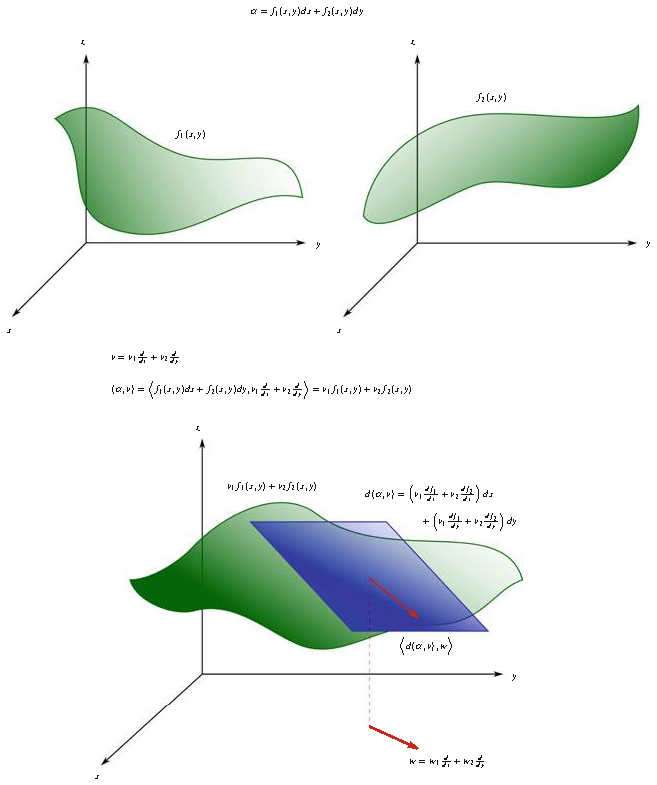
\includegraphics[width=0.960\linewidth]{images/vector/fig-4-1.pdf}
  \caption{流形 $\mathbb{R}^2$ 上的 1-形式 $\alpha(x,y)=f_1(x,y)dx+f_2(x,y)dy$ 由上面所示的两个函数 $f_1,f_2:\mathbb{R}^2\to\mathbb{R}$ 构成. 一旦我们给定流形 $\mathbb{R}^2$ 上的向量场 $v$（这里是常向量场 $v=v_1\partial_x+v_2\partial_y$）, 就可以用它求出实值函数 $\langle\alpha,v\rangle=v_1f_1+v_2f_2$, 它可以被看作两个函数 $f_1,f_2$ 的线性组合. 然后可以求这个函数在另一个给定向量 $w=w_1\partial_x+w_2\partial_y$ 方向上的方向导数. 这里微分 $d\langle\alpha,v\rangle$ 本质上编码了函数 $\langle\alpha,v\rangle$（以绿色显示）的切平面信息}
  \label{fig:4-1}
\end{figure}

总而言之, 我们这里有的
\[
d\langle\alpha,v\rangle(w)=v_1w_1\frac{\partial f_1}{\partial x}+v_2w_1\frac{\partial f_2}{\partial x}
+v_1w_2\frac{\partial f_1}{\partial y}+v_2w_2\frac{\partial f_2}{\partial y}
\]
是从流形 $\mathbb{R}^2$ 到 $\mathbb{R}$ 的函数. 当我们输入某个点 $p=(x_0,y_0)$ 时, 我们得到
\[
\begin{aligned}
d\langle\alpha_{(x_0,y_0)},v\rangle(w)
&=v_1w_1\left.\frac{\partial f_1(x,y)}{\partial x}\right|_{(x_0,y_0)}
+v_2w_1\left.\frac{\partial f_2(x,y)}{\partial x}\right|_{(x_0,y_0)}\\
&\qquad+v_1w_2\left.\frac{\partial f_1(x,y)}{\partial y}\right|_{(x_0,y_0)}
+v_2w_2\left.\frac{\partial f_2(x,y)}{\partial y}\right|_{(x_0,y_0)},
\end{aligned}
\]
这是一个数, 度量函数 $\langle\alpha,v\rangle=v_1f_1+v_2f_2$ 在给定点 $p=(x_0,y_0)$ 处沿向量 $w$ 移动时变化了多少.

这显然并不仅仅是度量 1-形式 $\alpha$ 如何变化. 相反, 它需要两个额外的向量 $v$ 和 $w$. 第一个向量 $v$ 与 1-形式一起用来构成实值函数 $\langle\alpha,v\rangle$, 然后用第二个向量来求这个函数的方向导数. 虽然这看起来是一种有点奇怪的度量 $\alpha$ 如何变化的方式, 但考虑到 1-形式作为一种数学对象实际上有多复杂, 这也许是我们能期望得到的最直截了当的方式了.

但在我们试图用这个公式以某种方式定义 1-形式 $\alpha$ 的微分之前, 我们决定谨慎一些, 看看当交换向量 $v$ 和 $w$ 的顺序时会发生什么. 也就是说, 我们想知道 $d\langle\alpha,w\rangle(v)$ 是什么. 毕竟, 如果我们简单地交换向量 $v$ 和 $w$ 的顺序, 我们会希望结果在某种意义上"相同". 继续这样做, 我们有 $\langle\alpha,w\rangle=w_1f_1+w_2f_2$, 这给出
\[
d\langle\alpha,w\rangle=\left(w_1\frac{\partial f_1}{\partial x}+w_2\frac{\partial f_2}{\partial x}\right)dx
+\left(w_1\frac{\partial f_1}{\partial y}+w_2\frac{\partial f_2}{\partial y}\right)dy,
\]
从而得到
\begin{align*}
d\langle\alpha,w\rangle(v)&=\bigl\langle d\langle\alpha,w\rangle,v\bigr\rangle\\
&=v_1w_1\frac{\partial f_1}{\partial x}+v_1w_2\frac{\partial f_2}{\partial x}
+v_2w_1\frac{\partial f_1}{\partial y}+v_2w_2\frac{\partial f_2}{\partial y}.
\end{align*}
让我们把这两个公式并排放在一起, 看看它们如何匹配.
\begin{align*}
\bigl\langle d\langle\alpha,v\rangle,w\bigr\rangle
&=v_1w_1\frac{\partial f_1}{\partial x}+v_2w_1\frac{\partial f_2}{\partial x}
+v_1w_2\frac{\partial f_1}{\partial y}+v_2w_2\frac{\partial f_2}{\partial y}\\
\bigl\langle d\langle\alpha,w\rangle,v\bigr\rangle
&=v_1w_1\frac{\partial f_1}{\partial x}+v_1w_2\frac{\partial f_2}{\partial x}
+v_2w_1\frac{\partial f_1}{\partial y}+v_2w_2\frac{\partial f_2}{\partial y}.
\end{align*}
所以, 这两个等式并不像我们可能希望的那样相同. 它们也不仅仅相差一个符号. 但显然 $d\langle\alpha,v\rangle(w)$ 与 $d\langle\alpha,w\rangle(v)$ 之间存在关系. 它们之间的关系要稍微复杂一些. 每个等式的第一项和最后一项是相同的, 但中间两项不同. 这两个公式都不能作为 1-形式导数的定义. 然而, 一切并没有失去. 一点巧妙的思考也许还能挽救局面.

在过去我们曾发现, 平行六面体的"体积"带有一个符号, 这个符号取决于向量的定向, 或者说顺序. 这种符号"歧义"已经出现在行列式的定义中, 然后出现在楔积的定义中. 因此, 如果我们最终确定的某种形式的导数的定义中出现这种符号, 我们也许不应过于惊讶或担心. 所以我们将使用一个在数学中时不时出现的"小技巧". 如果取这两项之差作为外微分的定义, 会发生什么？也就是说, 假设我们通过下面的公式定义 $\alpha$ 的外导数 $d\alpha$: 
\[
d\alpha(v,w)=\bigl\langle d\langle\alpha,w\rangle,v\bigr\rangle-\bigl\langle d\langle\alpha,v\rangle,w\bigr\rangle.
\]
用这个公式我们随后注意到, 交换 $v$ 和 $w$ 的顺序会改变符号, 
\begin{align*}
d\alpha(w,v)&=\bigl\langle d\langle\alpha,v\rangle,w\bigr\rangle-\bigl\langle d\langle\alpha,w\rangle,v\bigr\rangle\\
&=-\left(\bigl\langle d\langle\alpha,w\rangle,v\bigr\rangle-\bigl\langle d\langle\alpha,v\rangle,w\bigr\rangle\right)\\
&=-d\alpha(v,w).
\end{align*}
通过这样做, 我们得到 $d\alpha(v,w)$ 与 $d\alpha(w,v)$ 在相差一个符号的意义下给出相同的结果, 这是我们已经完全习惯并感到舒服的事情. 事实上, 考虑到符号在这个主题中的表现方式, 交换两个向量的顺序不改变某个东西的符号反而会令人惊讶. 所以, 我们将确定
\[
d\alpha(v,w)=\bigl\langle d\langle\alpha,w\rangle,v\bigr\rangle-\bigl\langle d\langle\alpha,v\rangle,w\bigr\rangle
\]
作为 $\alpha$ 的导数的工作定义. （实际上, 这个工作定义只在 $v$ 和 $w$ 恰好是常向量场时才有效, 但关于这一点我们稍后再说.）从几何上看, $d\alpha(v,w)$ 度量函数 $\langle\alpha,w\rangle$ 在 $v$ 方向上的变化减去函数 $\langle\alpha,v\rangle$ 在 $w$ 方向上的变化. 我们试图在图~\ref{fig:4-2} 中说明这一点.

\begin{figure}[htbp]
  \centering
  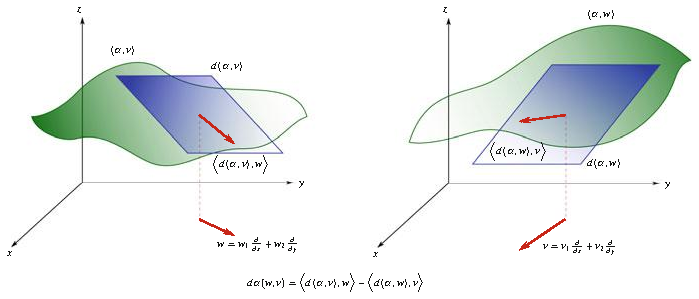
\includegraphics[width=0.960\linewidth]{images/vector/fig-4-2.pdf}
  \caption{左侧显示 $\langle\alpha,v\rangle$ 在 $w$ 方向上的变化, 右侧显示 $\langle\alpha,w\rangle$ 在 $v$ 方向上的变化. 这两个值之差随后被用来定义 $d\alpha(w,v)$. 这是度量 $\alpha$ 如何变化的一种间接方式}
  \label{fig:4-2}
\end{figure}

花点时间想想我们所做的. 由于 1-形式 $\alpha=f_1\,dx+f_2\,dy$ 是一个相当复杂的数学对象, 没有明显直接的方法度量它如何变化. 因此我们决定尝试用我们已经熟悉的技术, 即方向导数, 来间接度量 $\alpha$ 如何变化. 为了做到这一点, 我们需要两个（常）向量场 $v$ 和 $w$. 于是, 一旦我们给定了一个特定的 $v$ 和 $w$, 我们就用它们来间接度量 $\alpha$ 如何变化.

让我们用这个来得到 $d\alpha(v,w)$ 的实际表达式, 
\begin{align*}
d\alpha(v,w)&=\bigl\langle d\langle\alpha,w\rangle,v\bigr\rangle-\bigl\langle d\langle\alpha,v\rangle,w\bigr\rangle\\
&=v_1w_1\frac{\partial f_1}{\partial x}+v_1w_2\frac{\partial f_2}{\partial x}
+v_2w_1\frac{\partial f_1}{\partial y}+v_2w_2\frac{\partial f_2}{\partial y}\\
&\qquad-v_1w_1\frac{\partial f_1}{\partial x}-v_2w_1\frac{\partial f_2}{\partial x}
-v_1w_2\frac{\partial f_1}{\partial y}-v_2w_2\frac{\partial f_2}{\partial y}\\
&=v_1w_2\frac{\partial f_2}{\partial x}-v_1w_2\frac{\partial f_1}{\partial y}
-v_2w_1\frac{\partial f_2}{\partial x}+v_2w_1\frac{\partial f_1}{\partial y}\\
&=\left(\frac{\partial f_2}{\partial x}-\frac{\partial f_1}{\partial y}\right)(v_1w_2-w_1v_2)\\
&=\left(\frac{\partial f_2}{\partial x}-\frac{\partial f_1}{\partial y}\right)
\begin{vmatrix}v_1&w_1\\v_2&w_2\end{vmatrix}\\
&=\left(\frac{\partial f_2}{\partial x}-\frac{\partial f_1}{\partial y}\right)
\begin{vmatrix}dx(v)&dx(w)\\dy(v)&dy(w)\end{vmatrix}\\
&=\left(\frac{\partial f_2}{\partial x}-\frac{\partial f_1}{\partial y}\right)dx\wedge dy(v,w)\\
&=\left(\frac{\partial f_1}{\partial x}\underbrace{dx\wedge dx}_{=0}
+\frac{\partial f_1}{\partial y}\underbrace{dy\wedge dx}_{=-dx\wedge dy}
+\frac{\partial f_2}{\partial x}dx\wedge dy
+\frac{\partial f_2}{\partial y}\underbrace{dy\wedge dy}_{=0}\right)(v,w)\\
&=\Bigl(\underbrace{\left(\frac{\partial f_1}{\partial x}dx+\frac{\partial f_1}{\partial y}dy\right)}_{df_1}\wedge dx
+\underbrace{\left(\frac{\partial f_2}{\partial x}dx+\frac{\partial f_2}{\partial y}dy\right)}_{df_2}\wedge dy\Bigr)(v,w)\\
&=\bigl(df_1\wedge dx+df_2\wedge dy\bigr)(v,w).
\end{align*}
于是, 我们关于 $d\alpha$ 的"几何"定义——即函数 $\langle\alpha,w\rangle$ 在 $v$ 方向上的变化减去函数 $\langle\alpha,v\rangle$ 在 $w$ 方向上的变化——引导我们一路回到我们最初关于 $d\alpha$ 的公式 $\sum df_i\wedge dx_i$（当 $\alpha=\sum f_i\,dx_i$ 时）. 此外, 我们还有一个绝妙的额外收获: $d\alpha$ 结果是一个 2-形式. 好吧, 实际上这不仅仅是一个"额外收获". 这个定义导致 $d\alpha$ 是 2-形式这一事实, 正是我们确定这个（诚然有点笨拙的）1-形式外微分几何意义的首要原因.

实际上, 为了保持计算和图片的简单, 我们考察了流形 $\mathbb{R}^2$ 上的 1-形式 $\alpha$, 但我们本可以在任何流形上完成整个分析, 并得到同样的公式；只是计算会更麻烦一些.

我们意识到我们倾向于在不同记号之间跳来跳去, 而且我们将继续这样做. 我们实际上是故意这样做的, 让你习惯所有这些不同的记号很重要. 不同的书、论文和作者都倾向于使用不同的记号. 回顾 $df(v)=v[f]$ 以及 $\bigl\langle d\langle\alpha,w\rangle,v\bigr\rangle=v[\langle\alpha,w\rangle]$. 另外, 我们有 $\langle\alpha,w\rangle=\alpha(w)$, 所以我们可以把 $\bigl\langle d\langle\alpha,w\rangle,v\bigr\rangle$ 写成 $v[\alpha(w)]$. 类似地, 我们有 $\bigl\langle d\langle\alpha,v\rangle,w\bigr\rangle=w[\alpha(v)]$, 所以我们也可以把 $\alpha$ 的外导数（$v$ 和 $w$ 是常向量场）的定义写成
\begin{center}
\fbox{\parbox{0.86\textwidth}{\centering
\textbf{1-形式外微分的整体公式（常向量场）}\\[2pt]
$d\alpha(v,w)=\bigl\langle d\langle\alpha,w\rangle,v\bigr\rangle-\bigl\langle d\langle\alpha,v\rangle,w\bigr\rangle$
}}
\end{center}
或写成
\begin{center}
\fbox{\parbox{0.86\textwidth}{\centering
\textbf{1-形式外微分的整体公式（常向量场）}\\[2pt]
$d\alpha(v,w)=v[\alpha(w)]-w[\alpha(v)]$
}}
\end{center}

注意, 这正是我们在概述一节中给出的整体公式的前两项, 
\[
d\alpha(v,w)=v[\alpha(w)]-w[\alpha(v)]-\alpha([v,w]).
\]
于是我们看到, $d\alpha$ 的"几何"定义与 $d\alpha$ 的整体公式联系在一起. 然而, 我们缺少整体公式中的最后一项 $\alpha([v,w])$. 当 $v$ 和 $w$ 都是常向量场时这一项为零. 避开这一项的麻烦正是我们选择常向量场 $v$ 和 $w$ 的原因. 我们再次指出, 在这个整体公式中, 我们正在使用的实际坐标完全不出现. 这有时被称为坐标无关公式.

现在我们将对一个一般的 $n$ 维流形上的一般 1-形式快速重复这一过程. 这些计算适用于所谓的一般流形的坐标片. 这是我们将在后面某一章引入的概念, 所以现在只需想象我们在流形 $\mathbb{R}^n$ 上. 考虑 1-形式和向量
\[
\alpha=\sum_i\alpha_i\,dx_i,\qquad
v=\sum_i v_i\,\partial_{x_i},\qquad
w=\sum_i w_i\,\partial_{x_i}.
\]
于是我们有
\begin{align*}
\alpha(v)&=\langle\alpha,v\rangle\\
&=\left(\sum_i\alpha_i\,dx_i\right)\left(\sum_i v_i\,\partial_{x_i}\right)\\
&=\sum_i v_i\alpha_i.
\end{align*}
和以前一样, $\langle\alpha,v\rangle=\sum_i v_i\alpha_i$ 可以看作流形上的函数. 基本上, 这个函数是函数 $\alpha_i$ 以 $v_i$ 为权重的加权和. 使用在函数方向导数情形中定义的 $d$, 我们有
\begin{align*}
d\langle\alpha,v\rangle&=\sum_j\frac{\partial\left(\sum_i v_i\alpha_i\right)}{\partial x_j}dx_j\\
&=\sum_j\sum_i v_i\frac{\partial\alpha_i}{\partial x_j}dx_j.
\end{align*}
所以函数 $\langle\alpha,v\rangle=\sum_i v_i\alpha_i$ 在方向 $w$ 上的方向导数由下式给出
\begin{align*}
d\langle\alpha,v\rangle(w)&=\left(\sum_j\sum_i v_i\frac{\partial\alpha_i}{\partial x_j}dx_j\right)\left(\sum_k w_k\,\partial_{x_k}\right)\\
&=\sum_j\sum_i v_i\,w_j\frac{\partial\alpha_i}{\partial x_j}.
\end{align*}
回顾, 基本上 $d\langle\alpha,v\rangle$ 编码了函数 $\langle\alpha,v\rangle$ 的切空间, 而 $d\langle\alpha,v\rangle(w)$ 告诉我们沿 $w$ 移动时发生的变化. 一个完全相同的计算给出
\[
d\langle\alpha,w\rangle(v)=\sum_j\sum_i v_j\,w_i\frac{\partial\alpha_i}{\partial x_j}.
\]
比较 $d\langle\alpha,v\rangle(w)$ 和 $d\langle\alpha,w\rangle(v)$, 我们可以看到当 $i\neq j$ 时各项不同, 所以像以前一样, 我们定义
\begin{align*}
d\alpha(v,w)&=\bigl\langle d\langle\alpha,w\rangle,v\bigr\rangle-\bigl\langle d\langle\alpha,v\rangle,w\bigr\rangle\\
&=\sum_j\sum_i v_j\,w_i\frac{\partial\alpha_i}{\partial x_j}
-\sum_j\sum_i v_i\,w_j\frac{\partial\alpha_i}{\partial x_j}\\
&=\sum_j\sum_i\bigl(v_j\,w_i-v_i\,w_j\bigr)\frac{\partial\alpha_i}{\partial x_j}\\
&=\sum_j\sum_i\frac{\partial\alpha_i}{\partial x_j}
\begin{vmatrix}v_j&w_j\\v_i&w_i\end{vmatrix}\\
&=\sum_j\sum_i\frac{\partial\alpha_i}{\partial x_j}
\begin{vmatrix}dx_j(v)&dx_j(w)\\dx_i(v)&dx_i(w)\end{vmatrix}\\
&=\sum_j\sum_i\frac{\partial\alpha_i}{\partial x_j}dx_j\wedge dx_i\,(v,w)\\
&=\sum_i\left(\sum_j\frac{\partial\alpha_i}{\partial x_j}dx_j\right)\wedge dx_i\,(v,w)\\
&=\sum_i\underbrace{\left(\sum_j\frac{\partial\alpha_i}{\partial x_j}dx_j\right)}_{=d\alpha_i}\wedge dx_i\,(v,w).
\end{align*}
于是我们得到坐标内公式
\[
d\alpha=\sum_i d\alpha_i\wedge dx_i,
\]
这当然正是我们以前得到的.

与 1-形式的情形一样, 我们可以尝试为 $k$-形式 $\omega$ 的整体公式做一个几何论证. 第一步完全类似. 为了使用函数方向导数的概念, 我们必须通过放入不止一个而是 $k$ 个向量 $v_0,\ldots,v_{k-1}$ 把 $k$-形式变成一个函数, 然后我们度量这个函数在另一个向量 $v_k$ 方向上的变化. 然而, 下一步, 即我们实际使用数学"技巧"来定义 $d\omega$ 的那一步, 将很难合理化. 我们最终会得到
\begin{center}
\fbox{\parbox{0.86\textwidth}{\centering
\textbf{$k$-形式外微分的整体公式（常向量场）}\\[2pt]
$d\omega(v_0,\ldots,v_k)=\sum_i(-1)^i\bigl\langle d\bigl\langle\omega,(v_0,\ldots,\widehat{v_i},\ldots,v_k)\bigr\rangle,v_i\bigr\rangle$
}}
\end{center}
它也可以写成
\begin{center}
\fbox{\parbox{0.86\textwidth}{\centering
\textbf{$k$-形式外微分的整体公式（常向量场）}\\[2pt]
$d\omega(v_0,\ldots,v_k)=\sum_i(-1)^i\,v_i\bigl[\omega(v_0,\ldots,\widehat{v_i},\ldots,v_k)\bigr]$
}}
\end{center}
使用这个整体公式来得到坐标内公式也将是一个非常耗计算的过程. 因此我们将跳过它. 然而, 注意上面的公式与概述中的整体公式不同. 和以前一样, 这是因为我们使用的是常向量场.

\subsection{非常值向量场情形下的外微分}

我们对常向量场 $v$ 和 $w$ 所做的, 是作一些几何论证, 说明 $d\alpha(v,w)=v[\alpha(w)]-w[\alpha(v)]$ 会是用作 $\alpha$ 外微分整体公式的好定义. 然后我们用这个公式求出 1-形式 $\alpha=\sum_i\alpha_i\,dx_i$ 的外微分的坐标内公式, 发现它是 $d\alpha=\sum_i d\alpha_i\wedge dx_i$. 我们现在假设这就是我们想要的一般整体公式的坐标内形式.

由于我们并不是要给出外微分整体公式的实际证明, 而只是想让你对公式为什么是这样的以及如何成为这样的有一个感觉, 所以我们不会尝试逻辑上严谨的论证. 我们即将要做的实际上在逻辑上是反过来的. 我们知道我们想要得到的答案, 也就是说, 我们知道外导数的坐标内公式应该是什么, 所以我们将实际利用我们想最终到达哪里的知识, 来帮助我们找到并理解外微分的一般整体公式. 外微分的一般整体公式实际上将在第 A.7 节中以完全不同的方式证明, 使用附录中引入的许多概念和恒等式. 那节中的证明非常计算化, 公式似乎奇迹般地从各种配料的混合中冒出来. 本节则更脚踏实地, 给出动机, 并在更大程度上处理潜在的几何.

我们从 $\mathbb{R}^2$ 上的 1-形式 $\alpha$ 和两个非常值向量场 $v$、$w$ 开始, 
\[
\alpha=f_1\,dx+f_2\,dy,\qquad
v=g_1\,\partial_x+g_2\,\partial_y=\binom{g_1}{g_2},\qquad
w=h_1\,\partial_x+h_2\,\partial_y=\binom{h_1}{h_2},
\]
其中 $f_1,f_2,g_1,g_2,h_1,h_2$ 是流形 $\mathbb{R}^2$ 上的实值函数.

正如我们所说, 我们将从我们知道想得到的答案开始. 我们想要的 $\alpha$ 的外微分的坐标内公式是 $d\alpha=\sum_i d\alpha_i\wedge dx_i$. 所以我们首先计算它, 
\begin{align*}
d\alpha&=df_1\wedge dx+df_2\wedge dy\\
&=\left(\frac{\partial f_1}{\partial x}dx+\frac{\partial f_1}{\partial y}dy\right)\wedge dx
+\left(\frac{\partial f_2}{\partial x}dx+\frac{\partial f_2}{\partial y}dy\right)\wedge dy\\
&=\frac{\partial f_1}{\partial x}\underbrace{dx\wedge dx}_{=0}+\frac{\partial f_1}{\partial y}\underbrace{dy\wedge dx}_{=-dx\wedge dy}
+\frac{\partial f_2}{\partial x}dx\wedge dy+\frac{\partial f_2}{\partial y}\underbrace{dy\wedge dy}_{=0}\\
&=\left(\frac{\partial f_2}{\partial x}-\frac{\partial f_1}{\partial y}\right)dx\wedge dy.
\end{align*}
把我们的向量场 $v$ 和 $w$ 代进去, 我们得到
\begin{align*}
d\alpha(v,w)&=\left(\frac{\partial f_2}{\partial x}-\frac{\partial f_1}{\partial y}\right)dx\wedge dy(v,w)\\
&=\left(\frac{\partial f_2}{\partial x}-\frac{\partial f_1}{\partial y}\right)
\begin{vmatrix}dx(v)&dx(w)\\dy(v)&dy(w)\end{vmatrix}\\
&=\left(\frac{\partial f_2}{\partial x}-\frac{\partial f_1}{\partial y}\right)
\begin{vmatrix}g_1&h_1\\g_2&h_2\end{vmatrix}\\
&=\left(\frac{\partial f_2}{\partial x}-\frac{\partial f_1}{\partial y}\right)(g_1h_2-g_2h_1)\\
&=g_1h_2\frac{\partial f_2}{\partial x}-g_1h_2\frac{\partial f_1}{\partial y}
-g_2h_1\frac{\partial f_2}{\partial x}+g_2h_1\frac{\partial f_1}{\partial y}.
\end{align*}
到现在为止我们应该对这类计算感到舒服了. 唯一的区别是常数 $v_1,v_2,w_1,w_2$ 被函数 $g_1,g_2,h_1,h_2$ 取代了. 这就是我们想得到的答案. 稍后我们将回过头来参考这个等式.

我们的策略与常向量场情形相同, 出于同样的几何原因. 事实上, 基于常向量场情形, 我们首先猜想整体公式是 $d\alpha(v,w)=v[\alpha(w)]-w[\alpha(v)]$. 我们将做这个（诚然很乱的）计算, 发现它的项比上面求出的 $d\alpha(v,w)$ 的局部公式多得多. 然后我们将把这些项归并在一起, 并把它们称为 $\alpha([v,w])$, 从而对 1-形式的情形给出完整的整体公式 $d\alpha(v,w)=v[\alpha(w)]-w[\alpha(v)]-\alpha([v,w])$. 当然, 在那个时候你还不知道 $\alpha([v,w])$ 是什么. 然后我们将花一些时间解释这最后一项实际上表示什么. 括号 $[\,\cdot\,,\cdot\,]$（其中点被向量取代）被称为李括号, 所以 $[v,w]$ 是 $v$ 和 $w$ 的李括号, 结果它也是另一个向量场, 这很好, 因为它要被 1-形式 $\alpha$ 吞入.

现在我们准备开始了. 同样的论证适用. 我们想以某种方式度量 $\alpha$ 如何变化. 由于我们不确定如何做到这一点, 我们先把 $\alpha$ 变成我们知道如何研究的东西, 即一个函数, 这可以通过把它与向量场 $v$（它不再需要是常向量场）配对来完成, 
\[
\langle\alpha,v\rangle=[f_1,f_2]\binom{g_1}{g_2}=f_1g_1+f_2g_2.
\]
把这个与常向量场的情形相比较, 在那种情形中我们得到 $v_1f_1+v_2f_2$, 其中 $v_1$ 和 $v_2$ 是常数. 现在的情况立即更复杂了, 因为它涉及函数的乘积, 而不仅仅是函数的加权和.

为了求函数 $f_1g_1+f_2g_2$ 的方向导数, 我们首先求函数 $\langle\alpha,v\rangle$ 的微分, 
\begin{align*}
d\langle\alpha,v\rangle&=\frac{\partial(f_1g_1+f_2g_2)}{\partial x}dx+\frac{\partial(f_1g_1+f_2g_2)}{\partial y}dy\\
&=\left(\frac{\partial(f_1g_1)}{\partial x}+\frac{\partial(f_2g_2)}{\partial x}\right)dx
+\left(\frac{\partial(f_1g_1)}{\partial y}+\frac{\partial(f_2g_2)}{\partial y}\right)dy\\
&=\left(\frac{\partial f_1}{\partial x}\cdot g_1+f_1\cdot\frac{\partial g_1}{\partial x}
+\frac{\partial f_2}{\partial x}\cdot g_2+f_2\cdot\frac{\partial g_2}{\partial x}\right)dx\\
&\qquad+\left(\frac{\partial f_1}{\partial y}\cdot g_1+f_1\cdot\frac{\partial g_1}{\partial y}
+\frac{\partial f_2}{\partial y}\cdot g_2+f_2\cdot\frac{\partial g_2}{\partial y}\right)dy.
\end{align*}
注意, 这里需要使用乘积法则, 导致项的数目是我们以前处理常向量场时的两倍. 而且这些项本身也是函数的乘积. 这就是处理非常值向量场复杂得多的原因. 我们现在通过
\begin{align*}
\bigl\langle d\langle\alpha,v\rangle,w\bigr\rangle
&=\left(\frac{\partial f_1}{\partial x}\cdot g_1+f_1\cdot\frac{\partial g_1}{\partial x}
+\frac{\partial f_2}{\partial x}\cdot g_2+f_2\cdot\frac{\partial g_2}{\partial x}\right)h_1\\
&\qquad+\left(\frac{\partial f_1}{\partial y}\cdot g_1+f_1\cdot\frac{\partial g_1}{\partial y}
+\frac{\partial f_2}{\partial y}\cdot g_2+f_2\cdot\frac{\partial g_2}{\partial y}\right)h_2\\
&=g_1h_1\frac{\partial f_1}{\partial x}+f_1h_1\frac{\partial g_1}{\partial x}
+g_2h_1\frac{\partial f_2}{\partial x}+f_2h_1\frac{\partial g_2}{\partial x}\\
&\qquad+g_1h_2\frac{\partial f_1}{\partial y}+f_1h_2\frac{\partial g_1}{\partial y}
+g_2h_2\frac{\partial f_2}{\partial y}+f_2h_2\frac{\partial g_2}{\partial y}
\end{align*}
来求 $\langle\alpha,v\rangle$ 在 $w$ 方向上的方向导数.

接下来我们交换向量场 $v$ 和 $w$ 重复这个过程, 
\[
\langle\alpha,w\rangle=[f_1,f_2]\binom{h_1}{h_2}=f_1h_1+f_2h_2.
\]
为了求方向导数, 我们需要
\begin{align*}
d\langle\alpha,w\rangle&=\frac{\partial(f_1h_1+f_2h_2)}{\partial x}dx+\frac{\partial(f_1h_1+f_2h_2)}{\partial y}dy\\
&=\left(\frac{\partial(f_1h_1)}{\partial x}+\frac{\partial(f_2h_2)}{\partial x}\right)dx
+\left(\frac{\partial(f_1h_1)}{\partial y}+\frac{\partial(f_2h_2)}{\partial y}\right)dy\\
&=\left(\frac{\partial f_1}{\partial x}\cdot h_1+f_1\cdot\frac{\partial h_1}{\partial x}
+\frac{\partial f_2}{\partial x}\cdot h_2+f_2\cdot\frac{\partial h_2}{\partial x}\right)dx\\
&\qquad+\left(\frac{\partial f_1}{\partial y}\cdot h_1+f_1\cdot\frac{\partial h_1}{\partial y}
+\frac{\partial f_2}{\partial y}\cdot h_2+f_2\cdot\frac{\partial h_2}{\partial y}\right)dy.
\end{align*}
于是 $\langle\alpha,w\rangle$ 在 $v$ 方向上的方向导数由下式给出
\begin{align*}
\bigl\langle d\langle\alpha,w\rangle,v\bigr\rangle
&=\left(\frac{\partial f_1}{\partial x}\cdot h_1+f_1\cdot\frac{\partial h_1}{\partial x}
+\frac{\partial f_2}{\partial x}\cdot h_2+f_2\cdot\frac{\partial h_2}{\partial x}\right)g_1\\
&\qquad+\left(\frac{\partial f_1}{\partial y}\cdot h_1+f_1\cdot\frac{\partial h_1}{\partial y}
+\frac{\partial f_2}{\partial y}\cdot h_2+f_2\cdot\frac{\partial h_2}{\partial y}\right)g_2\\
&=h_1g_1\frac{\partial f_1}{\partial x}+f_1g_1\frac{\partial h_1}{\partial x}
+h_2g_1\frac{\partial f_2}{\partial x}+f_2g_1\frac{\partial h_2}{\partial x}\\
&\qquad+h_1g_2\frac{\partial f_1}{\partial y}+f_1g_2\frac{\partial h_1}{\partial y}
+h_2g_2\frac{\partial f_2}{\partial y}+f_2g_2\frac{\partial h_2}{\partial y}.
\end{align*}

回顾在我们的策略中, 我们首先猜想 $d\alpha(v,w)=v[\alpha(w)]-w[\alpha(v)]$. 在常向量情形中我们选择它, 仅仅因为它似乎是可行的, 而且它还导致交换向量 $v$ 和 $w$ 会改变符号这一事实. 按照我们的假设进行下去, 我们有
\begin{align*}
d\alpha(v,w)&=v[\alpha(w)]-w[\alpha(v)]\\
&\overset{\text{假设}}{=}\bigl\langle d\langle\alpha,w\rangle,v\bigr\rangle-\bigl\langle d\langle\alpha,v\rangle,w\bigr\rangle\\
&=h_1g_1\frac{\partial f_1}{\partial x}+f_1g_1\frac{\partial h_1}{\partial x}
+h_2g_1\frac{\partial f_2}{\partial x}+f_2g_1\frac{\partial h_2}{\partial x}
+h_1g_2\frac{\partial f_1}{\partial y}+f_1g_2\frac{\partial h_1}{\partial y}\\
&\qquad+h_2g_2\frac{\partial f_2}{\partial y}+f_2g_2\frac{\partial h_2}{\partial y}\\
&\qquad-g_1h_1\frac{\partial f_1}{\partial x}-f_1h_1\frac{\partial g_1}{\partial x}
-g_2h_1\frac{\partial f_2}{\partial x}-f_2h_1\frac{\partial g_2}{\partial x}
-g_1h_2\frac{\partial f_1}{\partial y}-f_1h_2\frac{\partial g_1}{\partial y}\\
&\qquad-g_2h_2\frac{\partial f_2}{\partial y}-f_2h_2\frac{\partial g_2}{\partial y}.
\end{align*}
注意, 有四项立刻消掉了. 由于我们已经知道我们想要的局部坐标内公式看起来是什么样, 现在我们转向它. 基于上面的计算, 我们试图到达的是
\[
d\alpha(v,w)=g_1h_2\frac{\partial f_2}{\partial x}-g_1h_2\frac{\partial f_1}{\partial y}
-g_2h_1\frac{\partial f_2}{\partial x}+g_2h_1\frac{\partial f_1}{\partial y}.
\]
因此我们有八个多余项
\[
f_1g_1\frac{\partial h_1}{\partial x}+f_2g_1\frac{\partial h_2}{\partial x}
+f_1g_2\frac{\partial h_1}{\partial y}+f_2g_2\frac{\partial h_2}{\partial y}
-f_1h_1\frac{\partial g_1}{\partial x}-f_2h_1\frac{\partial g_2}{\partial x}
-f_1h_2\frac{\partial g_1}{\partial y}-f_2h_2\frac{\partial g_2}{\partial y}.
\]
正如我们策略中所说的, 我们将把这些项归并在一起, 并把它们称为 $\alpha([v,w])$, 得到
\[
\begin{aligned}
\alpha([v,w])&=f_1g_1\frac{\partial h_1}{\partial x}+f_2g_1\frac{\partial h_2}{\partial x}
+f_1g_2\frac{\partial h_1}{\partial y}+f_2g_2\frac{\partial h_2}{\partial y}\\
&\qquad-f_1h_1\frac{\partial g_1}{\partial x}-f_2h_1\frac{\partial g_2}{\partial x}
-f_1h_2\frac{\partial g_1}{\partial y}-f_2h_2\frac{\partial g_2}{\partial y}.
\end{aligned}
\]
于是这反过来给出整体公式
\[
d\alpha(v,w)=v[\alpha(w)]-w[\alpha(v)]-\alpha([v,w]).
\]
当然, 在这一点上, 这个整体公式中的最后一项似乎只不过是一个记号上的方便；我们不知道它实际上表示什么. 事实是, 第三项确实表示某种几何上有趣而重要的东西, 我们现在就来解释.

两个向量场 $v$ 和 $w$ 的李括号的定义, 记为 $[v,w]$, 是根据这些向量场如何作用于函数 $F:\mathbb{R}^2\to\mathbb{R}$ 来定义的. 给定定义在流形 $\mathbb{R}^2$ 上的向量场 $w$, 我们可以求 $F$ 在 $w$ 方向上的方向导数. 在特定点 $p\in\mathbb{R}^2$ 处, $w_p[F]$ 是一个值, 告诉我们 $F$ 在点 $p$ 处沿 $w$ 方向变化有多快. 但如果我们不指定点 $p$, 那么 $w[F]$ 就是流形 $\mathbb{R}^2$ 上的另一个函数. 也就是说, 
\[
w[F]:\mathbb{R}^2\to\mathbb{R},\qquad p\longmapsto w_p[F].
\]
我们可以再次取这个函数 $w[F]$ 在 $v$ 方向上的方向导数. 同样, 在点 $p\in\mathbb{R}^2$ 处, $v_p[w[F]]$ 是一个值, 告诉我们 $w[F]$ 在点 $p$ 处沿 $v$ 方向变化有多快. 然而, 如果我们不指定点, 那么 $v[w[F]]$ 又是流形 $\mathbb{R}^2$ 上的另一个函数, 
\[
v[w[F]]:\mathbb{R}^2\to\mathbb{R},\qquad p\longmapsto v_p\bigl[w[F]\bigr].
\]

\begin{figure}[htbp]
  \centering
  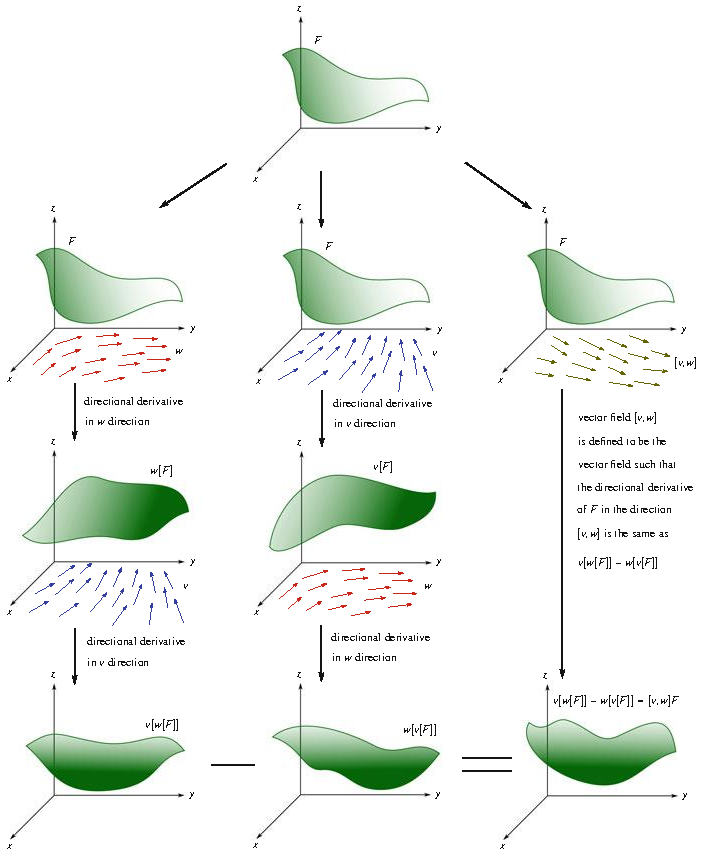
\includegraphics[width=0.960\linewidth]{images/vector/fig-4-3.pdf}
  \caption{在左侧, 我们取 $F:\mathbb{R}^2\to\mathbb{R}$ 在 $w$ 方向上的方向导数, 得到函数 $w[F]$, 然后再取 $w[F]$ 在 $v$ 方向上的方向导数, 得到函数 $v[w[F]]$. 在中间, 我们取 $F$ 在 $v$ 方向上的方向导数, 得到函数 $v[F]$, 然后再取 $v[F]$ 在 $w$ 方向上的方向导数, 得到 $w[v[F]]$. 取这两个函数之差 $v[w[F]]-w[v[F]]$, 得到一个新函数, 显示在底部. $v$ 和 $w$ 的李括号（记为 $[v,w]$）就是这样的向量场: 当应用于原始函数 $F$ 时, 它给出这个新函数. 换句话说, $[v,w]F=v[w[F]]-w[v[F]]$, 如右侧所示}
  \label{fig:4-3}
\end{figure}

这个过程全部在图~\ref{fig:4-3} 的左侧作了说明. 如果我们颠倒向量场的顺序, 先用 $v$, 我们得到函数 $v[F]:\mathbb{R}^2\to\mathbb{R}$. 接着应用 $w$, 我们得到函数 $w[v[F]]:\mathbb{R}^2\to\mathbb{R}$. 这个过程在图~\ref{fig:4-3} 的中部作了说明. 假设我们随后取这两个函数之差, 如图~\ref{fig:4-3} 的底部那样, 那么我们会得到一个新函数
\[
v\bigl[w[F]\bigr]-w\bigl[v[F]\bigr]:\mathbb{R}^2\to\mathbb{R}.
\]
事实上, 有可能找到一个单一的向量场, 一步完成这一切. 换句话说, 我们可以找到一个单一的向量场, 当应用于 $F$ 时恰好给出这个函数 $v[w[F]]-w[v[F]]$. 这个单一的向量场被称为 $v$ 和 $w$ 的李括号, 记为 $[v,w]$. 于是我们有
\[
[v,w]F=v\bigl[w[F]\bigr]-w\bigl[v[F]\bigr].
\]
这显示在图~\ref{fig:4-3} 的右侧. 尽管记号 $[v,w]$ 中包含两个向量场 $v$ 和 $w$, 但 $[v,w]$ 只是一个单一的向量场. 还要注意, 方括号有两种不同的用法. 然而, 通过注意方括号里面是什么, 应该很容易区分这两种用法. 我们将在下面用计算求出 $[v,w]$, 但应该指出, 还有一种看待 $[v,w]$ 的稍微几何化一点的方式. 事实上, 结果 $[v,w]$ 就是 $w$ 在 $v$ 方向上的李导数. 对这一点的解释留到第~\ref{sec:A-7} 节和图~\ref{fig:A-5}、\ref{fig:A-6}.

假设我们在记号中去掉函数 $F$, 得到
\[
[v,w]\,\cdot\,=v\bigl[w[\,\cdot\,]\bigr]-w\bigl[v[\,\cdot\,]\bigr].
\]
这解释了为什么你几乎总是会看到 $v$ 和 $w$ 的李括号被偷懒地定义为
\[
[v,w]=vw-wv.
\]

我们的目标现在转向确切找出向量场 $[v,w]$ 是什么, 
\begin{align*}
[v,w]F&=(vw-wv)F\\
&=v\bigl[w[F]\bigr]-w\bigl[v[F]\bigr]\\
&=v\left(h_1\frac{\partial F}{\partial x}+h_2\frac{\partial F}{\partial y}\right)
-w\left(g_1\frac{\partial F}{\partial x}+g_2\frac{\partial F}{\partial y}\right)\\
&=(g_1\partial_x+g_2\partial_y)\left(h_1\frac{\partial F}{\partial x}+h_2\frac{\partial F}{\partial y}\right)
-(h_1\partial_x+h_2\partial_y)\left(g_1\frac{\partial F}{\partial x}+g_2\frac{\partial F}{\partial y}\right)\\
&=g_1\frac{\partial}{\partial x}\left(h_1\frac{\partial F}{\partial x}\right)
+g_1\frac{\partial}{\partial x}\left(h_2\frac{\partial F}{\partial y}\right)
+g_2\frac{\partial}{\partial y}\left(h_1\frac{\partial F}{\partial x}\right)
+g_2\frac{\partial}{\partial y}\left(h_2\frac{\partial F}{\partial y}\right)\\
&\qquad-h_1\frac{\partial}{\partial x}\left(g_1\frac{\partial F}{\partial x}\right)
-h_1\frac{\partial}{\partial x}\left(g_2\frac{\partial F}{\partial y}\right)
-h_2\frac{\partial}{\partial y}\left(g_1\frac{\partial F}{\partial x}\right)
-h_2\frac{\partial}{\partial y}\left(g_2\frac{\partial F}{\partial y}\right)\\
&\overset{\text{积法则}}{=}g_1\frac{\partial h_1}{\partial x}\frac{\partial F}{\partial x}
+g_1h_1\frac{\partial^2 F}{\partial x^2}
+g_1\frac{\partial h_2}{\partial x}\frac{\partial F}{\partial y}
+g_1h_2\frac{\partial^2 F}{\partial x\partial y}\\
&\qquad+g_2\frac{\partial h_1}{\partial y}\frac{\partial F}{\partial x}
+g_2h_1\frac{\partial^2 F}{\partial y\partial x}
+g_2\frac{\partial h_2}{\partial y}\frac{\partial F}{\partial y}
+g_2h_2\frac{\partial^2 F}{\partial y^2}\\
&\qquad-h_1\frac{\partial g_1}{\partial x}\frac{\partial F}{\partial x}
-h_1g_1\frac{\partial^2 F}{\partial x^2}
-h_1\frac{\partial g_2}{\partial x}\frac{\partial F}{\partial y}
-h_1g_2\frac{\partial^2 F}{\partial x\partial y}\\
&\qquad-h_2\frac{\partial g_1}{\partial y}\frac{\partial F}{\partial x}
-h_2g_1\frac{\partial^2 F}{\partial y\partial x}
-h_2\frac{\partial g_2}{\partial y}\frac{\partial F}{\partial y}
-h_2g_2\frac{\partial^2 F}{\partial y^2}\\
&=g_1\frac{\partial h_1}{\partial x}\frac{\partial F}{\partial x}
+g_1\frac{\partial h_2}{\partial x}\frac{\partial F}{\partial y}
+g_2\frac{\partial h_1}{\partial y}\frac{\partial F}{\partial x}
+g_2\frac{\partial h_2}{\partial y}\frac{\partial F}{\partial y}\\
&\qquad-h_1\frac{\partial g_1}{\partial x}\frac{\partial F}{\partial x}
-h_1\frac{\partial g_2}{\partial x}\frac{\partial F}{\partial y}
-h_2\frac{\partial g_1}{\partial y}\frac{\partial F}{\partial x}
-h_2\frac{\partial g_2}{\partial y}\frac{\partial F}{\partial y}\\
&=\left(g_1\frac{\partial h_1}{\partial x}+g_2\frac{\partial h_1}{\partial y}
-h_1\frac{\partial g_1}{\partial x}-h_2\frac{\partial g_1}{\partial y}\right)\frac{\partial}{\partial x}[F]\\
&\qquad+\left(g_1\frac{\partial h_2}{\partial x}+g_2\frac{\partial h_2}{\partial y}
-h_1\frac{\partial g_2}{\partial x}-h_2\frac{\partial g_2}{\partial y}\right)\frac{\partial}{\partial y}[F]
\end{align*}
其中各项由于混合偏导数的相等而相消. 于是我们找到了向量场 $[v,w]$ 所取的形式, 它由下式给出
\[
[v,w]=\left(g_1\frac{\partial h_1}{\partial x}+g_2\frac{\partial h_1}{\partial y}
-h_1\frac{\partial g_1}{\partial x}-h_2\frac{\partial g_1}{\partial y}\right)\partial_x
+\left(g_1\frac{\partial h_2}{\partial x}+g_2\frac{\partial h_2}{\partial y}
-h_1\frac{\partial g_2}{\partial x}-h_2\frac{\partial g_2}{\partial y}\right)\partial_y
\]
即
\[
[v,w]=
\begin{bmatrix}
g_1\frac{\partial h_1}{\partial x}+g_2\frac{\partial h_1}{\partial y}-h_1\frac{\partial g_1}{\partial x}-h_2\frac{\partial g_1}{\partial y}\\[4pt]
g_1\frac{\partial h_2}{\partial x}+g_2\frac{\partial h_2}{\partial y}-h_1\frac{\partial g_2}{\partial x}-h_2\frac{\partial g_2}{\partial y}
\end{bmatrix}.
\]

现在让我们看看 $\alpha$ 作用于向量场 $[v,w]$ 是什么. 我们有
\begin{align*}
\alpha([v,w])&=\bigl\langle\alpha,[v,w]\bigr\rangle\\
&=[f_1,f_2]\begin{bmatrix}
g_1\frac{\partial h_1}{\partial x}+g_2\frac{\partial h_1}{\partial y}-h_1\frac{\partial g_1}{\partial x}-h_2\frac{\partial g_1}{\partial y}\\[4pt]
g_1\frac{\partial h_2}{\partial x}+g_2\frac{\partial h_2}{\partial y}-h_1\frac{\partial g_2}{\partial x}-h_2\frac{\partial g_2}{\partial y}
\end{bmatrix}\\
&=f_1g_1\frac{\partial h_1}{\partial x}+f_1g_2\frac{\partial h_1}{\partial y}
-f_1h_1\frac{\partial g_1}{\partial x}-f_1h_2\frac{\partial g_1}{\partial y}\\
&\qquad+f_2g_1\frac{\partial h_2}{\partial x}+f_2g_2\frac{\partial h_2}{\partial y}
-f_2h_1\frac{\partial g_2}{\partial x}-f_2h_2\frac{\partial g_2}{\partial y}.
\end{align*}
这里注意记号, $[v,w]$ 是两个向量场的李括号, 它本身是一个向量场, 而 $[f_1,f_2]$ 是与微分 1-形式 $\alpha=f_1\,dx+f_2\,dy$ 相联系的余向量, 即行向量. 区分这两个数学上不同的对象的方法是密切注意括号里面是什么: 向量场还是函数. 但注意我们得到的东西, 这八项正好就是 $v[\alpha(w)]-w[\alpha(v)]$ 中剩下的八项. 因此, 我们把流形 $\mathbb{R}^2$ 上 1-形式 $\alpha$ 的外微分的整体公式定义为
\[
d\alpha(v,w)=v[\alpha(w)]-w[\alpha(v)]-\alpha([v,w]).
\]

当然, 到目前为止我们只对流形 $\mathbb{R}^2$ 上的 1-形式做了这些. 流形 $\mathbb{R}^n$ 上的一般 1-形式又怎样呢？我们将同样走一遍这些（诚然相当复杂的）计算, 以确认一切都像预期的那样成立. 我们从
\[
\alpha=\sum_i\alpha_i\,dx_i,\qquad
v=\sum_i g_i\,\partial_{x_i},\qquad
w=\sum_i h_i\,\partial_{x_i}
\]
开始. 我们首先计算 $[v,w]$. 使用流形上的实值函数 $F$, 我们首先求出
\begin{align*}
v\bigl[w[F]\bigr]&=v\left(\sum_i h_i\frac{\partial F}{\partial x_i}\right)\\
&=\left(\sum_j g_j\,\partial_{x_j}\right)\left(\sum_i h_i\frac{\partial F}{\partial x_i}\right)\\
&=\sum_j g_j\,\partial_{x_j}\left(\sum_i h_i\frac{\partial F}{\partial x_i}\right)\\
&=\sum_j\sum_i g_j\left(\frac{\partial h_i}{\partial x_j}\cdot\frac{\partial F}{\partial x_i}
+h_i\frac{\partial}{\partial x_j}\left(\frac{\partial F}{\partial x_i}\right)\right)\\
&=\sum_j\sum_i\left(g_j\frac{\partial h_i}{\partial x_j}\cdot\frac{\partial F}{\partial x_i}
+g_jh_i\frac{\partial}{\partial x_j}\left(\frac{\partial F}{\partial x_i}\right)\right).
\end{align*}
求下一项是类似的, 我们得到
\[
w\bigl[v[F]\bigr]=\sum_j\sum_i\left(h_j\frac{\partial g_i}{\partial x_j}\cdot\frac{\partial F}{\partial x_i}
+h_jg_j\frac{\partial}{\partial x_j}\left(\frac{\partial F}{\partial x_i}\right)\right).
\]
把这两项放在一起, 我们得到
\begin{align*}
v\bigl[w[F]\bigr]-w\bigl[v[F]\bigr]
&=\sum_j\sum_i\left(g_j\frac{\partial h_i}{\partial x_j}\cdot\frac{\partial F}{\partial x_i}
+g_jh_i\frac{\partial}{\partial x_j}\left(\frac{\partial F}{\partial x_i}\right)\right)\\
&\qquad-\sum_j\sum_i\left(h_j\frac{\partial g_i}{\partial x_j}\cdot\frac{\partial F}{\partial x_i}
+h_jg_j\frac{\partial}{\partial x_j}\left(\frac{\partial F}{\partial x_i}\right)\right)\\
&=\sum_j\sum_i\left(g_j\frac{\partial h_i}{\partial x_j}-h_j\frac{\partial g_i}{\partial x_j}\right)\frac{\partial F}{\partial x_i}\\
&\qquad+\underbrace{\sum_i\sum_j g_jh_i\frac{\partial}{\partial x_j}\left(\frac{\partial F}{\partial x_i}\right)
-\sum_j\sum_i h_jg_j\frac{\partial}{\partial x_j}\left(\frac{\partial F}{\partial x_i}\right)}_{=0, \text{交换哑指标}}\\
&=\sum_i\left(\sum_j\left(g_j\frac{\partial h_i}{\partial x_j}-h_j\frac{\partial g_i}{\partial x_j}\right)\right)\frac{\partial F}{\partial x_i}.
\end{align*}
去掉函数 $F$ 我们得到实际的向量场
\[
[v,w]=\sum_i\left(\sum_j\left(g_j\frac{\partial h_i}{\partial x_j}-h_j\frac{\partial g_i}{\partial x_j}\right)\right)\partial_{x_i}.
\]
最后, 我们求出
\begin{align*}
\alpha([v,w])&=\left(\sum_k\alpha_k\,dx_k\right)
\left(\sum_i\left(\sum_j\left(g_j\frac{\partial h_i}{\partial x_j}-h_j\frac{\partial g_i}{\partial x_j}\right)\right)\partial_{x_i}\right)\\
&=\sum_i\alpha_i\left(\sum_j\left(g_j\frac{\partial h_i}{\partial x_j}-h_j\frac{\partial g_i}{\partial x_j}\right)\right).
\end{align*}
现在我们把注意力转向表达式 $v[\alpha(w)]-w[\alpha(v)]-\alpha([v,w])$. 由于
\[
v[\alpha(w)]=d(\alpha(v))(w)=\bigl\langle d(\alpha(v)),w\bigr\rangle
=\bigl\langle d\langle\alpha,v\rangle,w\bigr\rangle,
\]
我们从
\[
\langle\alpha,v\rangle=\left(\sum_i\alpha_i\,dx_i\right)\left(\sum_j g_j\,\partial_{x_j}\right)=\sum_i\alpha_i g_i
\]
开始. 求方向导数我们得到
\begin{align*}
d\langle\alpha,v\rangle&=d\left(\sum_i\alpha_i g_i\right)\\
&=\sum_j\frac{\partial\left(\sum_i\alpha_i g_i\right)}{\partial x_j}dx_j\\
&=\sum_j\sum_i\left(g_i\frac{\partial\alpha_i}{\partial x_j}+\alpha_i\frac{\partial g_i}{\partial x_j}\right)dx_j,
\end{align*}
然后用它求出
\[
w[\alpha(v)]=\sum_j\sum_i h_j\left(g_i\frac{\partial\alpha_i}{\partial x_j}+\alpha_i\frac{\partial g_i}{\partial x_j}\right).
\]
类似地我们有
\[
v[\alpha(w)]=\sum_j\sum_i g_j\left(h_i\frac{\partial\alpha_i}{\partial x_j}+\alpha_i\frac{\partial h_i}{\partial x_j}\right).
\]
接下来, 我们把一切组合起来
\begin{align*}
d\alpha(v,w)&=v[\alpha(w)]-w[\alpha(v)]-\alpha([v,w])\\
&=\sum_j\sum_i g_jh_i\frac{\partial\alpha_i}{\partial x_j}
+\sum_j\sum_i g_j\alpha_i\frac{\partial h_i}{\partial x_j}
-\sum_j\sum_i h_jg_i\frac{\partial\alpha_i}{\partial x_j}
-\sum_j\sum_i h_j\alpha_i\frac{\partial g_i}{\partial x_j}\\
&\qquad-\sum_i\alpha_i\sum_j\left(g_j\frac{\partial h_i}{\partial x_j}-h_j\frac{\partial g_i}{\partial x_j}\right)\\
&=\sum_{i,j}\bigl(g_jh_i-h_jg_i\bigr)\frac{\partial\alpha_i}{\partial x_j}
+\underbrace{\sum_{i,j}g_j\alpha_i\frac{\partial h_i}{\partial x_j}
-\sum_{i,j}\alpha_ig_j\frac{\partial h_i}{\partial x_j}}_{=0}\\
&\qquad\qquad+\underbrace{\sum_{i,j}h_j\alpha_i\frac{\partial g_i}{\partial x_j}
-\sum_{i,j}\alpha_ih_j\frac{\partial g_i}{\partial x_j}}_{=0}\\
&=\sum_{i,j}\bigl(g_jh_i-h_jg_i\bigr)\frac{\partial\alpha_i}{\partial x_j}\\
&=\sum_j\sum_i\frac{\partial\alpha_i}{\partial x_j}
\begin{vmatrix}g_j&h_j\\g_i&h_i\end{vmatrix}\\
&=\sum_j\sum_i\frac{\partial\alpha_i}{\partial x_j}
\begin{vmatrix}dx_j(v)&dx_j(w)\\dx_i(v)&dx_i(w)\end{vmatrix}\\
&=\sum_j\sum_i\frac{\partial\alpha_i}{\partial x_j}dx_j\wedge dx_i\,(v,w)\\
&=\sum_i\left(\sum_j\frac{\partial\alpha_i}{\partial x_j}dx_j\right)\wedge dx_i\,(v,w)\\
&=\sum_i\underbrace{\left(\sum_j\frac{\partial\alpha_i}{\partial x_j}dx_j\right)}_{=d\alpha_i}\\
&\qquad\qquad\qquad\wedge dx_i\,(v,w),
\end{align*}
这正是我们想要的坐标内公式 $d\alpha=\sum_i d\alpha_i\wedge dx_i$. 因此, 流形 $\mathbb{R}^n$ 上一般 1-形式的整体公式实际上正是我们想要的, 
\begin{center}
\fbox{\parbox{0.86\textwidth}{\centering
\textbf{1-形式外微分的整体公式}\\[2pt]
$d\alpha(v,w)=v[\alpha(w)]-w[\alpha(v)]-\alpha([v,w])$
}}
\end{center}

与常向量场的情形一样, 我们不会尝试为流形 $\mathbb{R}^n$ 上一般 $k$-形式的外微分整体公式提供几何论证. 这个过程将非常耗计算, 而且几何也一点也不清晰. 然而, 我们现在拥有了所需要的全部组成部分, 可以对公式为什么是这样的有一个整体的直观感觉. $k$-形式 $\omega$ 的外微分将是一个 $(k+1)$-形式, 这需要 $k+1$ 个输入向量场 $v_0,\ldots,v_k$. 我们从 0 开始编号, 仅仅是为了有一个简洁干净的 $(-1)^{i+j}$ 项, 
\begin{center}
\fbox{\parbox{0.88\textwidth}{\centering
\textbf{$k$-形式外微分的整体公式}\\[2pt]
$d\alpha(v_0,\ldots,v_k)=\sum_i(-1)^i\,v_i\bigl[\alpha(v_0,\ldots,\widehat{v_i},\ldots,v_k)\bigr]
+\sum_{i<j}(-1)^{i+j}\,\alpha\bigl([v_i,v_j],v_0,\ldots,\widehat{v_i},\ldots,\widehat{v_j},\ldots,v_k\bigr)$
}}
\end{center}
和以前一样, 记号中的帽子表示那些元素被省略. 这个公式实际上将在第 A.7 节被证明. 那里的证明将完全是计算性的, 并要求使用到那一章才会引入的概念和恒等式.

\begin{question}\label{q:4-5}
证明: 在 1-形式的情形下, $k$-形式外微分的整体公式约化为 1-形式外微分的整体公式.
\end{question}

\section{另一个几何观点}

我们以给出 $k$-形式 $\omega$ 的外微分的又一个定义来开始本节. 然后我们将证明, 使用这个定义我们恰好得到前面几节中 $d\omega$ 的同一个公式. 之后我们将考察这个定义的几何意义. 在许多方面, 这个定义给出了外导数最连贯、最易理解的几何表示, 遗憾的是更多的书不强调这种几何. 正如引言一节中提到的, 要真正理解外微分的这个定义, 需要先理解形式的积分. 而通常积分不在微分之前引入. 然而, 从某个角度看, 微分形式可以被看作"要积分的东西". 如果从这一角度来呈现微分形式, 那么积分就会被首先讨论.

基于你在微积分中对积分的理解, 你应该能够通过阅读本节对这些思想及其背后的几何获得一个大致的感受. 然而, 各种计算依赖于第 6 章至第 11 章中发展并给出的思想、记号和公式, 所以你不应该期望理解其中的细节. 在第一次阅读时, 只需试着理解大图景. 我们也强烈建议在第 11 章之后重新阅读本节.

我们将通过考察函数 $f$ 的导数的经典定义来为 $k$-形式 $\omega$ 的外微分的新定义提供动机. 回顾函数只不过是一个 0-形式. 我们有
\[
\frac{df(x)}{dx}=\lim_{h\to 0}\frac{1}{h}\Bigl(f(x+h)-f(x)\Bigr).
\]
我们在长度为 $h$ 的区间的端点处求 $f$ 的值, 该区间记为 $hP=[x,x+h]$. 这里的方括号表示 $\mathbb{R}$ 上的闭区间. 闭区间是包含端点的 $\mathbb{R}$ 上的区间. 出于第 10 章详细解释的原因, 区间 $hP$ 的边界（记为 $\partial(hP)$）是点 $\{(x+h)\}$ 减去点 $\{(x)\}$. 也就是说, $\partial(hP)=\partial[x,x+h]=\{(x+h)\}-\{(x)\}$. 虽然这是我们在微积分中通常不感兴趣、因此通常也不做的事情, 但我们可以把函数在单个点的积分定义为函数在该点的值. 于是
\[
\int_{\{(x+h)\}}f\equiv f(x+h)\qquad\text{和}\qquad
\int_{-\{(x)\}}f\equiv -f(x).
\]
注意来自 $-\{(x)\}$ 的负号发生了什么. 这使我们能够把 $f$ 的导数的定义改写为
\begin{align*}
\frac{df(x)}{dx}&=\lim_{h\to 0}\frac{1}{h}\Bigl(f(x+h)-f(x)\Bigr)\\
&=\lim_{h\to 0}\frac{1}{h}\left(\int_{\{(x+h)\}}f+\int_{-\{(x)\}}f\right)\\
&=\lim_{h\to 0}\frac{1}{h}\int_{\{(x+h)\}-\{(x)\}}f\\
&=\lim_{h\to 0}\frac{1}{h}\int_{\partial(hP)}f.
\end{align*}
于是我们把 0-形式 $f$ 的导数写成 $f$ 在一维平行六面体 $[x,x+h]$ 的边界上的积分. 在微积分中, 用最终等式后面的公式作为 $f$ 的导数的定义是荒谬的, 但对于微分形式来说, 这个定义导致了对外微分几何意义的清晰理解, 因此把这个公式（应用于 $k$-形式）作为定义是有意义的. 于是我们定义: 对流形 $\mathbb{R}^n$ 上的 $k$-形式 $\omega$, $\omega$ 在向量 $v_1,\ldots,v_{k+1}$ 的基点处的外微分为
\begin{center}
\fbox{\parbox{0.86\textwidth}{\centering
\textbf{$k$-形式的外微分}\\[2pt]
$d\omega\bigl(v_1,\ldots,v_{k+1}\bigr)=\lim_{h\to 0}\frac{1}{h^{k+1}}\int_{\partial(hP)}\omega$
}}
\end{center}
其中 $P$ 是由向量 $v_1,\ldots,v_{k+1}$ 张成的平行六面体, $hP$ 是该平行六面体按 $h$ 缩放得到的, $\partial(hP)$ 是缩放后的平行六面体的边界. 再说一遍, 平行六面体的边界是什么意思将在第 10 章详细解释.

在探索这个定义的几何意义之前, 我们将证明这个定义导致与前面几节中期望得到的完全相同的 $d\omega$ 公式. 在证明中, 我们不得不使用一些实际上在后面的章节中推导出来的概念、记号和公式. 我们还必须使用一些不在本书范围内、因此我们不加以解释或给出太多严谨性的想法和技术. 函数的 Taylor 级数就是这些想法之一. 在下面的推导中, 我们将简单地假设 Taylor 级数在点 $a$ 的某个邻域内收敛到给定的函数 $f$.

设 $f:\mathbb{R}^n\to\mathbb{R}$. $f$ 关于点 $a=(a_1,\ldots,a_n)$ 的 Taylor 级数由下式给出
\begin{align*}
f(x_1,\ldots,x_n)&=\sum_{i_1=0}^{\infty}\cdots\sum_{i_n=0}^{\infty}
\frac{(x_1-a_1)^{i_1}\cdots(x_n-a_n)^{i_n}}{i_1!\cdots i_n!}
\left.\frac{\partial^{i_1+\cdots+i_n}f}{\partial^{i_1}x_1\cdots\partial^{i_n}x_n}\right|_{(a_1,\ldots,a_n)}\\
&=f(a_1,\ldots,a_n)+\sum_{j=1}^{n}(x_j-a_j)\left.\frac{\partial f}{\partial x_j}\right|_{(a_1,\ldots,a_n)}\\
&\qquad+\frac{1}{2!}\sum_{j=0}^{n}\sum_{k=0}^{n}(x_j-a_j)(x_k-a_k)
\left.\frac{\partial^2 f}{\partial x_j\partial x_k}\right|_{(a_1,\ldots,a_n)}\\
&\qquad+\frac{1}{3!}\sum_{j=0}^{n}\sum_{k=0}^{n}\sum_{\ell=0}^{n}(x_j-a_j)(x_k-a_k)(x_\ell-a_\ell)
\left.\frac{\partial^3 f}{\partial x_j\partial x_k\partial x_\ell}\right|_{(a_1,\ldots,a_n)}\\
&\qquad+\cdots
\end{align*}
本质上, 对于充分接近点 $(a_1,\ldots,a_n)$ 的点 $(x_1,\ldots,x_n)$, 我们可以把 $f$ 改写成上述和.

\begin{question}\label{q:4-6}
证明 $f$ 的 Taylor 级数的这两个表示是相同的.
\end{question}

在求 $d\omega$ 的公式时, 我们将做两个简化调整. 第一, 我们在原点处写 $f$ 的 Taylor 级数, 因此有 $(a_1,\ldots,a_n)=(0,\ldots,0)$. 第二, 我们把所有二阶及更高阶的项归并成一个余项函数, 简单地记作 $R$. 于是我们的 Taylor 级数可以改写为
\[
f(x_1,\ldots,x_n)=f(0,\ldots,0)+\sum_{j=1}^{n}x_j\left.\frac{\partial f}{\partial x_j}\right|_{(0,\ldots,0)}+R(x_1,\ldots,x_n).
\]
接下来, 我们把流形 $\mathbb{R}^n$ 与向量空间 $\mathbb{R}^n$ 等同起来. 这将意味着下面的论证只适用于本身也是向量空间的流形, 不过加上我们在这里不关心的适当技术细节, 把结果推广到一般的 $n$ 维流形是可能的. 提供这些细节会使我们偏离大图景太远. 利用我们的等同, 我们有
\[
\text{流形 }\mathbb{R}^n\;\longleftrightarrow\;\text{向量空间 }\mathbb{R}^n,\qquad
p=(x_1,\ldots,x_n)\;\Longleftrightarrow\;v=\begin{bmatrix}x_1\\\vdots\\x_n\end{bmatrix}.
\]
注意, Taylor 级数的第二项可以写成
\[
\sum_{j=1}^{n}x_j\left.\frac{\partial f}{\partial x_j}\right|_{(0,\ldots,0)}
=\underbrace{\left(\left.\frac{\partial f}{\partial x_1}\right|_{(0,\ldots,0)},\cdots,
\left.\frac{\partial f}{\partial x_n}\right|_{(0,\ldots,0)}\right)}_{\text{余向量 }df_0}
\begin{bmatrix}x_1\\\vdots\\x_n\end{bmatrix}
=df_0(v),
\]
其中 $df$ 是 $f$ 通常的微分, 而 $df_0$ 是 $f$ 在原点 $(0,\ldots,0)=0$ 处取的微分. 由此我们可以把 Taylor 级数写在"点" $(x_1,\ldots,x_n)=v$ 处: 
\[
f(v)=f(0)+df_0(v)+R(v).
\]

现在, 假设我们给定向量 $v_1,\ldots,v_{k+1}$. 我们把由这些向量张成的平行六面体记为 $P$. 这里"张成"一词的用法与线性代数中的不同. 在这里我们有
\[
P=\mathrm{span}\{v_1,\ldots,v_{k+1}\}
=\left\{t_1v_1+\cdots+t_{k+1}v_{k+1}\;\middle|\;0\leq t_i\leq 1,\;i=1,\ldots,k+1\right\}.
\]
我们仍在把流形 $\mathbb{R}^n$ 与向量空间 $\mathbb{R}^n$ 等同, 因此向量 $t_1v_1+\cdots+t_{k+1}v_{k+1}$ 实际上指的是按照上述等同由该向量的坐标给出的点. 我们可以用因子 $h$ 缩放这个平行六面体, 得到新的平行六面体
\[
hP=\mathrm{span}\{hv_1,\ldots,hv_{k+1}\}
=\left\{t_1v_1+\cdots+t_{k+1}v_{k+1}\;\middle|\;0\leq t_i\leq h,\;i=1,\ldots,k+1\right\}.
\]
$hP$ 的各个面由下式给出
\[
hP_{(\ell,0)}=\left\{t_1v_1+\cdots+t_{\ell-1}v_{\ell-1}+0\,v_\ell+t_\ell v_{\ell+1}+\cdots+t_k v_{k+1}
\;\middle|\;0\leq t_i\leq h,\;i=1,\ldots,k\right\}
\]
或
\[
hP_{(\ell,1)}=\left\{t_1v_1+\cdots+t_{\ell-1}v_{\ell-1}+h\,v_\ell+t_\ell v_{\ell+1}+\cdots+t_k v_{k+1}
\;\middle|\;0\leq t_i\leq h,\;i=1,\ldots,k\right\},
\]
其中 $\ell=1,\ldots,k+1$. 注意 $t$ 的编号方式. 在 $hP$ 的各个面中, 我们现在有 $t_1$ 到 $t_k$. 继续把点写成向量, 面 $hP_{(\ell,1)}$ 和 $hP_{(\ell,0)}$ 的点可以分别写成
\[
v_{(\ell,1)}=hv_\ell+t_1v_1+\cdots+t_{\ell-1}v_{\ell-1}+t_\ell v_{\ell+1}+\cdots+t_k v_{k+1}
\]
和
\[
v_{(\ell,0)}=t_1v_1+\cdots+t_{\ell-1}v_{\ell-1}+t_\ell v_{\ell+1}+\cdots+t_k v_{k+1}.
\]
定义缩放的 $k$-立方体 $hI^k$ 为
\[
hI^k=\left\{(t_1,\ldots,t_k)\;\middle|\;0\leq t_i\leq h,\;i=1,\ldots,k\right\},
\]
只要我们知道向量 $v_1,\ldots,v_{k+1}$ 是什么, 那么对每个 $\ell$ 和任意值 $h$, 我们都在面 $hP_{(\ell,1)}$、$hP_{(\ell,0)}$ 与 $hI^k$ 之间有一个自然的等同, 
\[
hP_{(\ell,1)}\longleftrightarrow hI^k,\qquad v_{(\ell,1)}\longleftrightarrow (t_1,\ldots,t_k),
\]
以及
\[
hP_{(\ell,0)}\longleftrightarrow hI^k,\qquad v_{(\ell,0)}\longleftrightarrow (t_1,\ldots,t_k).
\]

我们现在将聚焦于 $hP_{(\ell,1)}\to hI^k$ 并仔细考察它. 我们在这个特殊情形中所做的对 $hP_{(\ell,0)}$ 和对所有 $\ell$ 也成立. 我们首先把这个映射命名为 $\Phi$, 于是我们有
\[
\Phi:\;hP_{(\ell,1)}\longrightarrow hI^k,\qquad v_{(\ell,1)}\longmapsto (t_1,\ldots,t_k).
\]
显然 $\Phi$ 是可逆的, 所以我们也有
\[
\Phi^{-1}:\;hP_{(\ell,1)}\longleftarrow hI^k,\qquad v_{(\ell,1)}\longmapsfrom (t_1,\ldots,t_k).
\]
如果我们给定一个点 $t=(t_1,\ldots,t_k)\in hI^k$, 那么我们可以写 $\Phi^{-1}(t)=v_{(\ell,1)}(t)$. 换句话说, 点 $v_{(\ell,1)}$ 被写成点 $t$ 的函数.

给定映射 $\Phi$, 我们还有切映射, 也称为\newterm{push-forward}{前推}{push-forward}, $T\Phi$. 当我们考虑切映射时, 我们实际上是把元素 $v_{(\ell,1)}$ 看作向量. $\Phi$ 的伴随切映射是
\[
T\Phi:\;T\bigl(hP_{(\ell,1)}\bigr)\longrightarrow T\bigl(hI^k\bigr),\qquad
v_{(\ell,1)}\longmapsto T\Phi\cdot v_{(\ell,1)}=\begin{bmatrix}t_1\\\vdots\\t_k\end{bmatrix}.
\]
我们特别感兴趣的是原来用来定义平行六面体 $P$ 的向量 $v_1,\ldots,v_{k+1}$ 发生了什么, 
\[
v_m\longmapsto T\Phi\cdot v_m=\begin{bmatrix}0\\\vdots\\1\\0\\\vdots\end{bmatrix}.
\]
对于 $T\Phi\cdot v_m$, 如果 $m<\ell$, 1 在第 $m$ 个槽位；如果 $m>\ell$, 则在第 $(m-1)$ 个槽位.

\begin{question}\label{q:4-7}
求 $T\Phi^{-1}\cdot e_i$, $i=1,\ldots,k$, 其中 $e_i$ 是标准欧几里得向量.
\end{question}

我们还有 $\Phi^{-1}$ 的余切映射, 也称为\newterm{pull-back}{拉回}{pull-back}, 
\[
T^*\Phi^{-1}:\;\Omega^k\bigl(hP_{(\ell,1)}\bigr)\longrightarrow\Omega^k\bigl(hI^k\bigr),\qquad
\alpha\longmapsto T^*\Phi^{-1}\cdot\alpha.
\]
我们特别感兴趣的是 $hP_{(\ell,1)}$ 上的 $k$-形式. 注意, $hP_{(\ell,1)}$ 是 $\mathbb{R}^{k+1}$ 的 $k$ 维子流形. 由于 $\mathbb{R}^{k+1}$ 已经有笛卡尔坐标函数 $x_1,\ldots,x_{k+1}$, 我们将简单地把它们用作嵌入子流形 $hP_{(\ell,1)}$ 的坐标函数. 这可能看起来有点奇怪, 因为流形 $hP_{(\ell,1)}$ 是 $k$ 维的, 而我们却在它上面使用 $k+1$ 个坐标函数. 但这是最简单的方法, 因为所讨论的流形不过是嵌入欧几里得空间的平行六面体, 我们对它非常了解. 另外, 我们将使用 $t_1,\ldots,t_k$ 作为 $hI^k$ 上的坐标函数. 本质上, $t_i$ 就是 $\mathbb{R}^k$ 上的笛卡尔坐标函数, 而 $hI^k$ 嵌入其中. 我们首先考察 $hP_{(\ell,1)}$ 上的 $k$-形式基元素, 
\[
dx_{i_1}\wedge\cdots\wedge dx_{i_k}.
\]
由于 $hP_{(\ell,1)}$ 和 $hI^k$ 都是 $k$ 维的, 我们知道 $T^*\Phi^{-1}\cdot\bigl(dx_{i_1}\wedge\cdots\wedge dx_{i_k}\bigr)$ 必定具有 $F\,dt_1\wedge\cdots\wedge dt_k$ 的形式. 注意 $\Omega^k\bigl(hI^k\bigr)$ 的维数是 1, 所以 $dt_1\wedge\cdots\wedge dt_k$ 是这个空间的基, 因而是 $hI^k$ 上的\newterm{volume-form}{体积形式}{volume form}. 我们想求出 $F$. 我们有
\begin{align*}
F&=F\,dt_1\wedge\cdots\wedge dt_k\,(e_1,\ldots,e_k)\\
&=\Bigl(T^*\Phi^{-1}\cdot\bigl(dx_{i_1}\wedge\cdots\wedge dx_{i_k}\bigr)\Bigr)(e_1,\ldots,e_k)\\
&=dx_{i_1}\wedge\cdots\wedge dx_{i_k}\Bigl(T\Phi^{-1}\cdot e_1,\ldots,T\Phi^{-1}\cdot e_{\ell-1},
T\Phi^{-1}\cdot e_\ell,\ldots,T\Phi^{-1}\cdot e_k\Bigr)\\
&=dx_{i_1}\wedge\cdots\wedge dx_{i_k}\Bigl(\underbrace{T\Phi^{-1}\cdot e_1}_{v_1},\ldots,
\underbrace{T\Phi^{-1}\cdot e_{\ell-1}}_{v_{\ell-1}},
\underbrace{T\Phi^{-1}\cdot e_\ell}_{v_{\ell+1}},\ldots,
\underbrace{T\Phi^{-1}\cdot e_k}_{v_{k+1}}\Bigr)\\
&=dx_{i_1}\wedge\cdots\wedge dx_{i_k}\bigl(v_1,\ldots,\widehat{v_\ell},\ldots,v_{k+1}\bigr).
\end{align*}
换句话说, 我们有 $F=dx_{i_1}\wedge\cdots\wedge dx_{i_k}\bigl(v_1,\ldots,\widehat{v_\ell},\ldots,v_{k+1}\bigr)$, 因此
\[
T^*\Phi^{-1}\cdot\bigl(dx_{i_1}\wedge\cdots\wedge dx_{i_k}\bigr)
=dx_{i_1}\wedge\cdots\wedge dx_{i_k}\bigl(v_1,\ldots,\widehat{v_\ell},\ldots,v_{k+1}\bigr)\,dt_1\wedge\cdots\wedge dt_k.
\]

在第 7 章中, 我们发展出下列涉及换元法的积分公式: 
\[
\int_{R}f(x_1,\ldots,x_n)\,dx_1\wedge\cdots\wedge dx_n
=\int_{\Phi(R)}f\circ\Phi^{-1}(\Phi_1,\ldots,\Phi_n)\,T^*\Phi^{-1}\cdot dx_1\wedge\cdots\wedge dx_n.
\]
我们现在将考虑这个公式如何应用于积分区域为 $hP_{(\ell,1)}$、换元映射为 $\Phi:hP_{(\ell,1)}\to hI^k$ 的情形. 把点 $(x_1,\ldots,x_k)$ 写成 $v_{(\ell,1)}$, 把点 $(t_1,\ldots,t_k)$ 写成 $t$, 回顾 $\Phi^{-1}(t)=v_{(\ell,1)}(t)$, 并把 $dx_{i_1}\wedge\cdots\wedge dx_{i_k}$ 写成 $dx^I$, 我们有
\begin{align*}
\int_{hP_{(\ell,1)}}f\bigl(v_{(\ell,1)}\bigr)\,dx_{i_1}\wedge\cdots\wedge dx_{i_k}
&=\int_{\Phi\bigl(hP_{(\ell,1)}\bigr)}f\circ\Phi^{-1}(t)\,T^*\Phi^{-1}\cdot\bigl(dx_{i_1}\wedge\cdots\wedge dx_{i_k}\bigr)\\
&=\int_{hI^k}f\bigl(v_{(\ell,1)}(t)\bigr)\,dx^I\bigl(v_1,\ldots,\widehat{v_\ell},\ldots,v_{k+1}\bigr)\,dt_1\wedge\cdots\wedge dt_k\\
&=\underbrace{\int_0^h\cdots\int_0^h}_{k\text{ 次}}
f\bigl(v_{(\ell,1)}(t)\bigr)\,dx^I\bigl(v_1,\ldots,\widehat{v_\ell},\ldots,v_{k+1}\bigr)\!\underbrace{dt\cdots dt}_{k\text{ 次}}.
\end{align*}
区域 $hP_{(\ell,0)}$ 的计算以及所有其他 $\ell$ 值的计算完全类似.

现在我们有了全部材料, 可以考虑本节开头给出的 $\omega$ 的外微分的定义. 对流形 $\mathbb{R}^n$ 上的 $k$-形式 $\omega$, $\omega$ 在向量 $v_1,\ldots,v_{k+1}$ 的基点处的外微分被定义为
\[
d\omega\bigl(v_1,\ldots,v_{k+1}\bigr)=\lim_{h\to 0}\frac{1}{h^{k+1}}\int_{\partial(hP)}\omega.
\]
为了简化计算, 我们在讨论 Taylor 级数展开时已经假设这个基点是流形 $\mathbb{R}^n$ 的原点. 如果我们感兴趣的点不是原点, 我们就必须平移 $k$-形式, 使我们感兴趣的点与原点重合, 做必要的计算, 然后再平移回去. 这会给我们要给出的论证增加一层复杂性, 但不会从根本上改变任何东西. 本质上, 我们通过只看一个特例来简化论证, 而这个特例经过一点额外的工作可以推广到一般情形. 在这种情形下数学中常用的一句话是不失一般性. 因此我们将说不失一般性地假设基点是原点.

考虑单位 $(k+1)$-立方体 $I^{k+1}$. 在第 11 章中我们求出 $I^{k+1}$ 的边界为
\[
\partial I^{k+1}=\sum_{i=1}^{k+1}\sum_{a=0}^{1}(-1)^{i+a}I_{(i,a)}^{k+1},
\]
其中 $I_{(i,a)}^{k+1}$ 是把第 $i$ 个变量固定为 $a$（$a$ 为 $0$ 或 $1$）所得到的 $I^{k+1}$ 的面. $(-1)^{i+a}$ 表示该面的定向. 这样, 彼此相对的两个面的定向相反. 任何平行六面体的边界都可以类似地求出, 因此我们有
\begin{align*}
\partial(hP)&=\sum_{\ell=1}^{k+1}\sum_{a=0}^{1}(-1)^{\ell+a}hP_{(\ell,a)}\\
&=\sum_{\ell=1}^{k+1}\Bigl((-\!1)^{\ell}hP_{(\ell,0)}+(-1)^{\ell+1}hP_{(\ell,1)}\Bigr).
\end{align*}
最后, 回顾函数 $f$ 关于原点的 Taylor 级数. 对接近原点的点 $v$ 有 $f(v)=f(0)+df_0(v)+R(v)$. 现在假设我们给定 $k$-形式 $\omega=f\,dx_{i_1}\wedge\cdots\wedge dx_{i_k}$, 那么外微分定义右端的积分可以写成
\begin{align*}
\int_{\partial(hP)}\omega&=\int_{\partial(hP)}f\,dx_{i_1}\wedge\cdots\wedge dx_{i_k}\\
&=\int_{\sum_{\ell=1}^{k+1}\bigl((-\!1)^{\ell}hP_{(\ell,0)}+(-1)^{\ell+1}hP_{(\ell,1)}\bigr)}
\underbrace{f\,dx_{i_1}\wedge\cdots\wedge dx_{i_k}}_{dx^I}\\
&=\sum_{\ell=1}^{k+1}\left((-\!1)^{\ell}\int_{hP_{(\ell,0)}}f\,dx^I+(-1)^{\ell+1}\int_{hP_{(\ell,1)}}f\,dx^I\right)\\
&=\sum_{\ell=1}^{k+1}(-1)^{\ell-1}\left(\int_{hP_{(\ell,1)}}f\,dx^I-\int_{hP_{(\ell,0)}}f\,dx^I\right)\\
&=\sum_{\ell=1}^{k+1}(-1)^{\ell-1}\Bigl(\int_{hP_{(\ell,1)}}\Bigl(f(0)+df_0(v)+R(v)\Bigr)dx^I\\
&\qquad\qquad\qquad\qquad-\int_{hP_{(\ell,0)}}\Bigl(f(0)+df_0(v)+R(v)\Bigr)dx^I\Bigr)\\
&=\sum_{\ell=1}^{k+1}(-1)^{\ell-1}\left(\int_{hP_{(\ell,1)}}f(0)\,dx^I-\int_{hP_{(\ell,0)}}f(0)\,dx^I\right)\tag{1}\\
&\qquad+\sum_{\ell=1}^{k+1}(-1)^{\ell-1}\\
&\qquad\qquad\Bigl(\int_{hP_{(\ell,1)}}df_0(v)\,dx^I-\int_{hP_{(\ell,0)}}df_0(v)\,dx^I\Bigr)\tag{2}\\
&+\sum_{\ell=1}^{k+1}(-1)^{\ell-1}\\
&\qquad\qquad\Bigl(\int_{hP_{(\ell,1)}}R(v)\,dx^I\\
&\qquad\qquad\qquad\qquad-\int_{hP_{(\ell,0)}}R(v)\,dx^I\Bigr).\tag{3}
\end{align*}

考虑出现在 (1) 中的第一项和第二项. 对每个 $\ell=1,\ldots,k+1$ 我们有
\begin{align*}
\int_{hP_{(\ell,1)}}f(0)\,dx^I-\int_{hP_{(\ell,0)}}f(0)\,dx^I
&=\int_{hI^k}f(0)\,dx^I\bigl(v_1,\ldots,\widehat{v_\ell},\ldots,v_{k+1}\bigr)\,dt_1\wedge\cdots\wedge dt_k\\
&\qquad-\int_{hI^k}f(0)\,dx^I\bigl(v_1,\ldots,\widehat{v_\ell},\ldots,v_{k+1}\bigr)\,dt_1\wedge\cdots\wedge dt_k\\
&=\int_{hI^k}\Bigl(\underbrace{f(0)}_{\text{常数}}-\underbrace{f(0)}_{\text{同一个常数}}\Bigr)\\
&\qquad\qquad dx^I\bigl(v_1,\ldots,\widehat{v_\ell},\ldots,v_{k+1}\bigr)\,dt_1\wedge\cdots\wedge dt_k\\
&=0.
\end{align*}
现在考虑出现在 (2) 中的第三项和第四项. 对每个 $\ell=1,\ldots,k+1$ 我们有
\begin{align*}
&\int_{hP_{(\ell,1)}}df_0(v)\,dx^I-\int_{hP_{(\ell,0)}}df_0(v)\,dx^I\\
&=\int_{hI^k}df_0\bigl(v_{(\ell,1)}(t)\bigr)\,dx^I\bigl(v_1,\ldots,\widehat{v_\ell},\ldots,v_{k+1}\bigr)\,dt_1\wedge\cdots\wedge dt_k\\
&\qquad-\int_{hI^k}df_0\bigl(v_{(\ell,0)}(t)\bigr)\,dx^I\bigl(v_1,\ldots,\widehat{v_\ell},\ldots,v_{k+1}\bigr)\,dt_1\wedge\cdots\wedge dt_k\\
&=\int_{hI^k}\Bigl(df_0\bigl(v_{(\ell,1)}(t)\bigr)-df_0\bigl(v_{(\ell,0)}(t)\bigr)\Bigr)dx^I\bigl(v_1,\ldots,\widehat{v_\ell},\ldots,v_{k+1}\bigr)\,dt_1\wedge\cdots\wedge dt_k\\
&=\int_{hI^k}\Bigl(df_0\bigl(hv_\ell+v_{(\ell,0)}(t)\bigr)-df_0\bigl(v_{(\ell,0)}(t)\bigr)\Bigr)dx^I\bigl(v_1,\ldots,\widehat{v_\ell},\ldots,v_{k+1}\bigr)\,dt_1\wedge\cdots\wedge dt_k\\
&=\int_{hI^k}\Bigl(\underbrace{df_0(hv_\ell)+df_0\bigl(v_{(\ell,0)}(t)\bigr)-df_0\bigl(v_{(\ell,0)}(t)\bigr)}_{=0}\Bigr)dx^I\bigl(v_1,\ldots,\widehat{v_\ell},\ldots,v_{k+1}\bigr)\,dt_1\wedge\cdots\wedge dt_k\\
&=\int_{hI^k}df_0(hv_\ell)\,dx^I\bigl(v_1,\ldots,\widehat{v_\ell},\ldots,v_{k+1}\bigr)\,dt_1\wedge\cdots\wedge dt_k\\
&=df_0(hv_\ell)\,dx^I\bigl(v_1,\ldots,\widehat{v_\ell},\ldots,v_{k+1}\bigr)\int_{hI^k}dt_1\wedge\cdots\wedge dt_k\\
&=df_0(hv_\ell)\,dx^I\bigl(v_1,\ldots,\widehat{v_\ell},\ldots,v_{k+1}\bigr)\underbrace{\int_0^h\cdots\int_0^h}_{k\text{ 次}}dt\cdots dt\\
&=h\,df_0(v_\ell)\,dx^I\bigl(v_1,\ldots,\widehat{v_\ell},\ldots,v_{k+1}\bigr)\cdot h^k\\
&=h^{k+1}df_0(v_\ell)\,dx^I\bigl(v_1,\ldots,\widehat{v_\ell},\ldots,v_{k+1}\bigr).
\end{align*}
现在我们考虑出现在 (3) 中的第五项和第六项: 
\begin{align*}
\int_{hP_{(\ell,1)}}R(v)\,dx^I-\int_{hP_{(\ell,0)}}R(v)\,dx^I
&=\int_{hI^k}R\bigl(v_{(\ell,1)}(t)\bigr)\,dx^I\bigl(v_1,\ldots,\widehat{v_\ell},\ldots,v_{k+1}\bigr)\\
&\qquad\qquad\cdot dt_1\wedge\cdots\wedge dt_k\\
&\qquad-\int_{hI^k}R\bigl(v_{(\ell,0)}(t)\bigr)\,dx^I\bigl(v_1,\ldots,\widehat{v_\ell},\ldots,v_{k+1}\bigr)\\
&\qquad\qquad\cdot dt_1\wedge\cdots\wedge dt_k\\
&=\int_{hI^k}\Bigl(R\bigl(v_{(\ell,1)}(t)\bigr)-R\bigl(v_{(\ell,0)}(t)\bigr)\Bigr)\\
&\qquad\qquad\cdot dx^I\bigl(v_1,\ldots,\widehat{v_\ell},\ldots,v_{k+1}\bigr)\,dt_1\wedge\cdots\wedge dt_k.
\end{align*}
我们只会以足够让你获得直观理解的详细程度来勾画论证的下一部分. 要填补论证的细节需要一些分析的背景, 而这是本书不假设读者具备的. 考虑在这种情形下余项到底是什么: 
\[
\begin{aligned}
R(x_1,\ldots,x_n)&=\frac{1}{2!}\sum_{j=0}^{n}\sum_{k=0}^{n}(x_j)(x_k)\left.\frac{\partial^2 f}{\partial x_j\partial x_k}\right|_{(0,\ldots,0)}\\
&\qquad+\frac{1}{3!}\sum_{j=0}^{n}\sum_{k=0}^{n}\sum_{m=0}^{n}(x_j)(x_k)(x_m)\left.\frac{\partial^3 f}{\partial x_j\partial x_k\partial x_m}\right|_{(0,\ldots,0)}+\cdots.
\end{aligned}
\]
我们把点 $(x_1,\ldots,x_n)$ 写成向量, 它要么是
\[
v_{(\ell,1)}=hv_\ell+t_1v_1+\cdots+t_{\ell-1}v_{\ell-1}+t_\ell v_{\ell+1}+\cdots+t_k v_{k+1}
\]
要么是
\[
v_{(\ell,0)}=t_1v_1+\cdots+t_{\ell-1}v_{\ell-1}+t_\ell v_{\ell+1}+\cdots+t_k v_{k+1}.
\]
有 $k+1$ 个向量, 每个由 $n$ 个分量组成. 取这 $n(k+1)$ 个分量的绝对值并找出最大值, 把它称为 $M$. 向量 $v_{(\ell,1)}$ 或 $v_{(\ell,0)}$ 中每个分量的绝对值都小于 $h(k+1)M$, 所以我们有
\[
\begin{aligned}
\bigl|R(x_1,\ldots,x_n)\bigr|&\leq\frac{1}{2!}\sum_{j=0}^{n}\sum_{k=0}^{n}\\
&\qquad\qquad\qquad\left|h(k+1)M\cdot h(k+1)M\left.\frac{\partial^2 f}{\partial x_j\partial x_k}\right|_{(0,\ldots,0)}\right|\\
&\qquad+\frac{1}{3!}\sum_{j=0}^{n}\sum_{k=0}^{n}\sum_{m=0}^{n}\\
&\qquad\qquad\qquad\left|h(k+1)M\cdot h(k+1)M\cdot h(k+1)M\left.\frac{\partial^3 f}{\partial x_j\partial x_k\partial x_m}\right|_{(0,\ldots,0)}\right|\\
&\qquad\qquad\qquad\qquad+\cdots.
\end{aligned}
\]
注意, 我们能够从这个和中的每一项中至少提出一个 $h^2$. 证明需要一些努力, 我们就不去做了, 但存在某个数 $K$ 使得
\[
\bigl|R(x_1,\ldots,x_n)\bigr|\leq h^2K.
\]
利用三角不等式, 我们有
\begin{align*}
\bigl|R\bigl(v_{(\ell,1)}(t)\bigr)-R\bigl(v_{(\ell,0)}(t)\bigr)\bigr|
&\leq\bigl|R\bigl(v_{(\ell,1)}(t)\bigr)\bigr|+\bigl|R\bigl(v_{(\ell,0)}(t)\bigr)\bigr|\\
&\leq h^2K+h^2K\\
&=2h^2K.
\end{align*}
类似地, 对某个值 $C$ 我们有
\begin{align*}
\bigl|dx^I\bigl(v_1,\ldots,\widehat{v_\ell},\ldots,v_{k+1}\bigr)\bigr|
&=\left|\sum_{\sigma\in S_k}\mathrm{sgn}(\sigma)\prod_{\substack{j=1\\j\neq\ell}}^{k+1}dx_{\sigma(i_j)}(v_j)\right|\\
&\leq\sum_{\sigma\in S_k}\prod_{\substack{j=1\\j\neq\ell}}^{k+1}\bigl|dx_{\sigma(i_j)}(v_j)\bigr|\\
&\leq C.
\end{align*}
把这一切放在一起, 
\begin{align*}
&\left|\int_{hI^k}\Bigl(R\bigl(v_{(\ell,1)}(t)\bigr)-R\bigl(v_{(\ell,0)}(t)\bigr)\Bigr)\right.\\
&\qquad\qquad\left.\vphantom{\int_{hI^k}}dx^I\bigl(v_1,\ldots,\widehat{v_\ell},\ldots,v_{k+1}\bigr)\,dt_1\wedge\cdots\wedge dt_k\right|\\
&\leq\int_{hI^k}2h^2KC\,dt_1\wedge\cdots\wedge dt_k\\
&=h^2(2KC)\underbrace{\int_0^h\cdots\int_0^h}_{k\text{ 次}}dt\cdots dt\\
&=h^{k+2}(2KC).
\end{align*}
回到我们离开的地方继续原来的计算, 
\begin{align*}
\int_{\partial(hP)}\omega&=\sum_{\ell=1}^{k+1}(-1)^{\ell-1}\left(\int_{hP_{(\ell,1)}}f(0)\,dx^I-\int_{hP_{(\ell,0)}}f(0)\,dx^I\right)\\
&\qquad+\sum_{\ell=1}^{k+1}(-1)^{\ell-1}\left(\int_{hP_{(\ell,1)}}df_0(v)\,dx^I-\int_{hP_{(\ell,0)}}df_0(v)\,dx^I\right)\\
&\qquad+\sum_{\ell=1}^{k+1}(-1)^{\ell-1}\left(\int_{hP_{(\ell,1)}}R(v)\,dx^I-\int_{hP_{(\ell,0)}}R(v)\,dx^I\right)\\
&\overset{\text{``=''}}{=}\sum_{\ell=1}^{k+1}(-1)^{\ell-1}\left(0+h^{k+1}df_0(v_\ell)\,dx^I\bigl(v_1,\ldots,\widehat{v_\ell},\ldots,v_{k+1}\bigr)+h^{k+2}(2KC)\right).
\end{align*}
严格来说, 由于我们得到 $h^{k+2}(2KC)$ 项的方式, 最后一个等式并不是等式, 但正如我们马上会看到的, 这没有关系. 把它用在 $d\omega$ 的定义中, 我们有
\begin{align*}
d\omega\bigl(v_1,\ldots,v_{k+1}\bigr)
&=\lim_{h\to 0}\frac{1}{h^{k+1}}\int_{\partial(hP)}\omega\\
&=\lim_{h\to 0}\frac{1}{h^{k+1}}\sum_{\ell=1}^{k+1}(-1)^{\ell-1}\\
&\qquad\qquad\left(0+h^{k+1}df_0(v_\ell)\,dx^I\bigl(v_1,\ldots,\widehat{v_\ell},\ldots,v_{k+1}\bigr)+h^{k+2}(2KC)\right)\\
&=\underbrace{\lim_{h\to 0}\sum_{\ell=1}^{k+1}(-1)^{\ell-1}\frac{0}{h^{k+1}}}_{=0}\\
&\qquad+\underbrace{\lim_{h\to 0}\sum_{\ell=1}^{k+1}(-1)^{\ell-1}df_0(v_\ell)\,dx^I\bigl(v_1,\ldots,\widehat{v_\ell},\ldots,v_{k+1}\bigr)}_{\text{不含 }h}\\
&\qquad+\underbrace{\lim_{h\to 0}\sum_{\ell=1}^{k+1}(-1)^{\ell-1}\frac{h^{k+2}}{h^{k+1}}(2KC)}_{\to 0}\\
&=\sum_{\ell=1}^{k+1}(-1)^{\ell-1}df_0(v_\ell)\,dx_{i_1}\wedge\cdots\wedge dx_{i_k}\bigl(v_1,\ldots,\widehat{v_\ell},\ldots,v_{k+1}\bigr)\\
&=df\wedge dx_{i_1}\wedge\cdots\wedge dx_{i_k}\bigl(v_1,\ldots,v_{k+1}\bigr),
\end{align*}
其中最后一行省去了基点 0. 下一个问题要求你证明最后一个等式.

\begin{question}\label{q:4-8}
使用 $k$-形式 $\alpha$ 与 $\ell$-形式 $\beta$ 的楔积用 $(k+\ell)$-\newterm{shuffle}{洗牌}{shuffle}给出的定义
\[
(\alpha\wedge\beta)\bigl(v_1,\ldots,v_{k+\ell}\bigr)
=\sum_{\sigma\text{ 是 }(k+\ell)\text{-洗牌}}\mathrm{sgn}(\sigma)\,
\alpha\bigl(v_{\sigma(1)},\ldots,v_{\sigma(k)}\bigr)\beta\bigl(v_{\sigma(k+1)},\ldots,v_{\sigma(k+\ell)}\bigr),
\]
证明上述计算中的最后一个等式.
\end{question}

于是我们证明了, 对 $\omega=f\,dx_{i_1}\wedge\cdots\wedge dx_{i_k}$, 外微分的这个定义导致与前面几节相同的计算公式. 那么显然很容易证明, 对一般的 $k$-形式 $\alpha=\sum \alpha_{i_1\cdots i_k}dx_{i_1}\wedge\cdots\wedge dx_{i_k}$, 有
\[
d\alpha=\sum d\alpha_{i_1\cdots i_k}\wedge dx_{i_1}\wedge\cdots\wedge dx_{i_k}.
\]

现在我们转而探索这个定义的几何. 为了能够画图, 我们将考察流形 $\mathbb{R}^3$ 上的一个 2-形式. 我们可以写
\begin{align*}
d\omega(v_1,v_2,v_3)&=\lim_{h\to 0}\frac{1}{h^3}\int_{\partial(hP)}\omega\\
&=\lim_{h\to 0}\frac{1}{h^3}\left(\int_{hP_{(1,1)}}\omega-\int_{hP_{(1,0)}}\omega
-\int_{hP_{(2,1)}}\omega+\int_{hP_{(2,0)}}\omega\right.\\
&\qquad\qquad\qquad\qquad\qquad\qquad\left.+\int_{hP_{(3,1)}}\omega-\int_{hP_{(3,0)}}\omega\right)\\
&=\lim_{h\to 0}\frac{1}{h^3}\underbrace{\left(\int_{hP_{(1,1)}}\omega-\int_{hP_{(1,0)}}\omega\right)}_{\text{见图~\ref{fig:4-4}}}\\
&\qquad-\lim_{h\to 0}\frac{1}{h^3}\underbrace{\left(\int_{hP_{(2,1)}}\omega-\int_{hP_{(2,0)}}\omega\right)}_{\text{见图~\ref{fig:4-5}}}\\
&\qquad+\lim_{h\to 0}\frac{1}{h^3}\underbrace{\left(\int_{hP_{(3,1)}}\omega-\int_{hP_{(3,0)}}\omega\right)}_{\text{见图~\ref{fig:4-5}}}.
\end{align*}
图~\ref{fig:4-4} 试图说明上面前两项发生的情况. 图中显示了由 $hv_1,hv_2,hv_3$ 张成的平行六面体 $hP$ 的两个面 $hP_{(1,0)}$ 和 $hP_{(1,1)}$. 这些面定义为
\[
hP_{(1,0)}=\left\{0\,v_1+t_2v_2+t_3v_3\;\middle|\;0\leq t_i\leq h,\;i=2,3\right\}
\]
以及
\[
hP_{(1,1)}=\left\{h\,v_1+t_2v_2+t_3v_3\;\middle|\;0\leq t_i\leq h,\;i=2,3\right\}.
\]
定义在 $\mathbb{R}^3$ 上的 2-形式 $\omega$ 在这两个二维空间中的每一个上积分. 利用我们对积分作用的直觉, 我们可以非常粗略地把这想成 $\omega$ 在这两个空间中的每一个上各自的"总量". 当我们取这些积分之差 $\int_{hP_{(1,1)}}\omega-\int_{hP_{(1,0)}}\omega$ 时, 我们是在试图度量 $\omega$ 的"总量"在我们沿 $v_1$ 方向移动时变化了多少. 当然, 我们得到的 $\omega$ 的"总量"依赖于我们积分的空间, 而这些空间是平行六面体 $hP$ 的面, 而 $hP$ 本身只是 $P$ 的缩小版. 因此, 方向 $v_1$ 和我们积分的面都依赖于原来的平行六面体 $P$. 我们说这两个积分之差给出了 $\omega$ 的"总量"相对于平行六面体 $P$ 在 $v_1$ 方向变化的度量.

\begin{figure}[htbp]
  \centering
  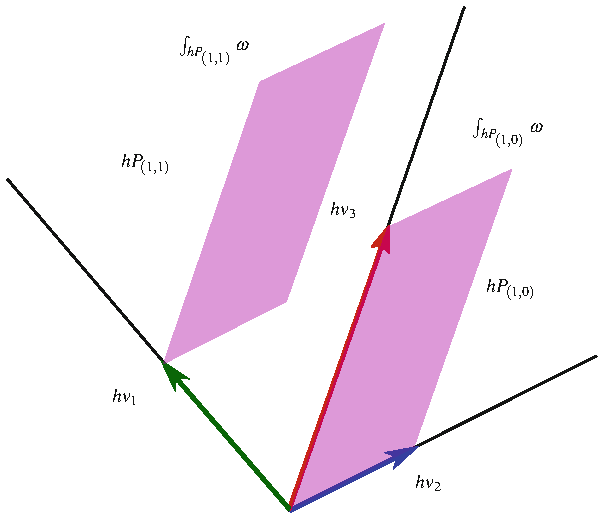
\includegraphics[width=0.803\linewidth]{images/vector/fig-4-4.pdf}
  \caption{这里显示了由 $hv_1,hv_2,hv_3$ 张成的平行六面体 $hP$ 的两个面 $hP_{(1,0)}$ 和 $hP_{(1,1)}$. 2-形式 $\omega$ 在这两个面上分别积分. 这两个积分之差 $\int_{hP_{(1,1)}}\omega-\int_{hP_{(1,0)}}\omega$ 给出 $\omega$ 的"总量"在 $v_1$ 方向变化的度量. 由于显然我们积分所用的 $hP$ 的面以及度量变化所用的方向 $v_1$ 都依赖于 $P$, 我们说我们度量的是 $\omega$ 的"总量"相对于 $P$ 在 $v_1$ 方向上的变化}
  \label{fig:4-4}
\end{figure}

\begin{figure}[htbp]
  \centering
  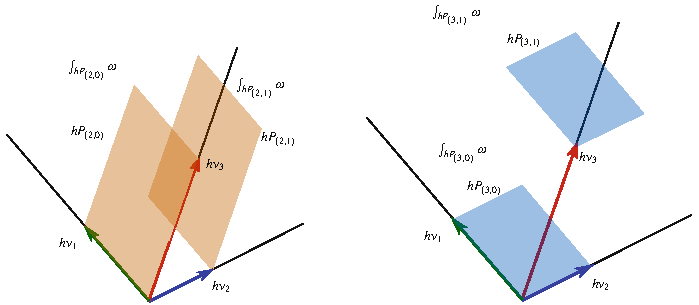
\includegraphics[width=0.960\linewidth]{images/vector/fig-4-5.pdf}
  \caption{在左侧, 我们求两个积分之差 $\int_{hP_{(2,1)}}\omega-\int_{hP_{(2,0)}}\omega$, 它给出 $\omega$ 的"总量"相对于 $P$ 在 $v_2$ 方向变化的度量. 类似地, 在右侧, 我们求两个积分之差 $\int_{hP_{(3,1)}}\omega-\int_{hP_{(3,0)}}\omega$, 它给出 $\omega$ 的"总量"相对于 $P$ 在 $v_3$ 方向变化的度量}
  \label{fig:4-5}
\end{figure}

以类似的方式, 积分之差 $\int_{hP_{(2,1)}}\omega-\int_{hP_{(2,0)}}\omega$ 给出 $\omega$ 的"总量"相对于平行六面体 $P$ 在 $v_2$ 方向变化的度量, 而积分之差 $\int_{hP_{(3,1)}}\omega-\int_{hP_{(3,0)}}\omega$ 给出 $\omega$ 的"总量"相对于平行六面体 $P$ 在 $v_3$ 方向变化的度量. 见图~\ref{fig:4-5}.

通过取 $\frac{1}{h^3}\left(\int_{hP_{(1,1)}}\omega-\int_{hP_{(1,0)}}\omega\right)$ 当 $h\to 0$ 时的极限, 我们实际上是在求 $\omega$ 的"总量"相对于 $P$ 在基点处沿 $v_1$ 方向的变化率. （回顾, 在上面的计算中, 我们曾不失一般性地假设向量 $v_1,\ldots,v_k$ 的基点是原点, 但一般来说基点可以是流形上的任意点.）$\frac{1}{h^3}\left(\int_{hP_{(2,1)}}\omega-\int_{hP_{(2,0)}}\omega\right)$ 和 $\frac{1}{h^3}\left(\int_{hP_{(3,1)}}\omega-\int_{hP_{(3,0)}}\omega\right)$ 当 $h\to 0$ 时的极限也分别求出 $\omega$ 的"总量"在基点处相对于由向量 $v_1,v_2,v_3$ 张成的平行六面体 $P$ 沿 $v_2$、$v_3$ 方向的变化率. 然后在此基础上, 我们把各种变化率相加/相减. 是加还是减按照 $P$ 各面的定向进行. 这将在第 11 章详细解释.

我们在特定点对 $d\omega(v_1,v_2,v_3)$ 实际得到的数, 是 $\omega$ 的"总量"在 $v_1$、$v_2$、$v_3$ 方向的各种变化率的某种奇怪的组合, 其中那些"总量"是用由向量 $v_1,v_2,v_3$ 张成的平行六面体的面来计算的. 因此数 $d\omega(v_1,v_2,v_3)$ 是 $\omega$ 的"总量"在基点处的一个总变化率, 它依赖于 $v_1,v_2,v_3$. 最终的这个数对你来说可能看起来有点奇怪, 但求它的所有组成部分都有非常清晰合理的几何意义. 当然, $d\omega$ 本身是一个 3-形式, 它使我们能够通过在给定点代入三个向量 $v_1,v_2,v_3$ 来计算该点的这个总变化率.

除了对"$\omega$ 的总量"这个说法获得一种感受之外, 使用这个定义给出了 $k$-形式外微分最具体的几何意义. 我们并没有试图在这里解释我们说"$\omega$ 的总量"是什么意思, 除了简单地说它是 $\omega$ 在 $P$ 的一个面上的积分. 形式的积分将在第 7 章至第 11 章解释. 特别是, 我们将在第 7.2 节从 Riemann 和的角度考察形式的积分, 这让我们对形式的积分在做什么有一个非常好的想法. 然而, 在三维情形中, 形式的积分有一些非常好的几何图景, 可以用来获得对正在发生之事的直观理解. 这些图景依赖于 1-形式、2-形式和 3-形式如何被可视化（这在第 5 章讨论）, 以及 Stokes 定理（在第 11 章讨论）. 我们将在第 11.6 节末尾回到对 1-形式、2-形式和 3-形式外微分几何的探索. 虽然对 $k>3$ 不再有帮助我们可视化微分形式的漂亮图景, 但 $n$ 维流形上 $k$-形式外微分的几何意义是类似的；只是需要考虑更多方向和 $P$ 的面, 而且 $P$ 的所有面都是 $k$ 维的.

$n$-形式 $\omega$ 的外微分的这个特定定义也给出了广义 Stokes 定理为什么成立的最清晰的直观想法. 使用这个定义, 
\begin{align*}
d\omega\bigl(v_1,\ldots,v_{k+1}\bigr)=\lim_{h\to 0}\frac{1}{h^{k+1}}\int_{\partial(hP)}\omega \\
\Longleftrightarrow
\end{align*}
当 $h$ 非常小时, 
\begin{align*}
d\omega\bigl(v_1,\ldots,v_{k+1}\bigr)\approx\frac{1}{h^{k+1}}\int_{\partial(hP)}\omega \\
\Longleftrightarrow
\end{align*}
两边同乘以 $h^{k+1}$, 
\begin{align*}
\underbrace{h^{k+1}}_{\text{一个数}}d\omega\bigl(v_1,\ldots,v_{k+1}\bigr)\approx\int_{\partial(hP)}\omega \\
\Longleftrightarrow
\end{align*}
$hP$ 的体积近似为 $h^{k+1}$, 
\begin{align*}
d\omega\bigl(v_1,\ldots,v_{k+1}\bigr)\underbrace{\int_{hP}dx_1\wedge\cdots\wedge dx_{k+1}}_{\text{体积形式}}\approx\int_{\partial(hP)}\omega \\
\Longleftrightarrow
\end{align*}
把这个数放到积分号里面, 
\begin{align*}
\int_{hP}d\omega\bigl(v_1,\ldots,v_{k+1}\bigr)\,dx_1\wedge\cdots\wedge dx_{k+1}\approx\int_{\partial(hP)}\omega \\
\Longleftrightarrow
\end{align*}
把左端写成抽象记号, 
\begin{align*}
\int_{hP}d\omega\approx\int_{\partial(hP)}\omega \\
\Longleftrightarrow
\end{align*}
令 $h\to 0$, 
\[
\int_{hP}d\omega=\int_{\partial(hP)}\omega.
\]
最后的蕴含给出区域 $hP$ 上的广义 Stokes 定理. 这当然不是一个严格的证明, 那在第 11 章完成, 但它的确提供了广义 Stokes 定理是什么的一个非常好的大图景, 以及它为什么成立的合理几何论证.

\begin{question}\label{q:4-9}
类似于上面的讨论, 解释 $n$ 维流形上 3-形式 $\omega$ 的 $d\omega(v_1,v_2,v_3,v_4)$ 的几何意义.
\end{question}

\begin{question}\label{q:4-10}
类似于上面的讨论, 解释 $n$ 维流形上 $k$-形式 $\omega$ 的 $d\omega(v_1,\ldots,v_k)$ 的几何意义.
\end{question}

\section{外微分例题}

现在我们转而利用前面几节得到的各种公式. 习惯外微分运算最简单的方式可能就是看一系列例子并亲手算一遍. 做这些计算时, 我们将相当详细, 只是为了让你习惯并熟悉一切. 一旦你熟悉了这类计算, 你就可以毫无问题地跳过许多步骤.

设我们有两个函数 $f,g:\mathbb{R}^2\to\mathbb{R}$. 我们想求 $df\wedge dg$. 首先我们注意到有
\[
df=\frac{\partial f}{\partial x}dx+\frac{\partial f}{\partial y}dy
\qquad\text{和}\qquad
dg=\frac{\partial g}{\partial x}dx+\frac{\partial g}{\partial y}dy.
\]
然后我们取这两个 1-形式的楔积, 并使用第 3.3.1 节给出的楔积的代数性质: 
\begin{align*}
df\wedge dg&=\left(\frac{\partial f}{\partial x}dx+\frac{\partial f}{\partial y}dy\right)
\wedge\left(\frac{\partial g}{\partial x}dx+\frac{\partial g}{\partial y}dy\right)\\
&=\frac{\partial f}{\partial x}dx\wedge\left(\frac{\partial g}{\partial x}dx+\frac{\partial g}{\partial y}dy\right)
+\frac{\partial f}{\partial y}dy\wedge\left(\frac{\partial g}{\partial x}dx+\frac{\partial g}{\partial y}dy\right)\\
&=\frac{\partial f}{\partial x}\frac{\partial g}{\partial x}\underbrace{dx\wedge dx}_{=0}
+\frac{\partial f}{\partial x}\frac{\partial g}{\partial y}dx\wedge dy
+\frac{\partial f}{\partial y}\frac{\partial g}{\partial x}dy\wedge dx
+\frac{\partial f}{\partial y}\frac{\partial g}{\partial y}\underbrace{dy\wedge dy}_{=0}\\
&=\frac{\partial f}{\partial x}\frac{\partial g}{\partial y}dx\wedge dy
+\frac{\partial f}{\partial y}\frac{\partial g}{\partial x}dy\wedge dx\\
&=\frac{\partial f}{\partial x}\frac{\partial g}{\partial y}dx\wedge dy
-\frac{\partial f}{\partial y}\frac{\partial g}{\partial x}dx\wedge dy\\
&=\left(\frac{\partial f}{\partial x}\frac{\partial g}{\partial y}-\frac{\partial f}{\partial y}\frac{\partial g}{\partial x}\right)dx\wedge dy\\
&=\begin{vmatrix}\frac{\partial f}{\partial x}&\frac{\partial f}{\partial y}\\[4pt]\frac{\partial g}{\partial x}&\frac{\partial g}{\partial y}\end{vmatrix}dx\wedge dy.
\end{align*}
所以, $df$ 和 $dg$ 的楔积在二维体积形式（面积形式）$dx\wedge dy$ 前面带有来自向量微积分的 Jacobian 矩阵. 换句话说, 我们找到了恒等式
\[
df\wedge dg=\underbrace{\begin{vmatrix}\frac{\partial f}{\partial x}&\frac{\partial f}{\partial y}\\[4pt]\frac{\partial g}{\partial x}&\frac{\partial g}{\partial y}\end{vmatrix}}_{\text{Jacobian 矩阵}}\underbrace{dx\wedge dy}_{\text{面积形式}}.
\]

证明对 $f,g,h:\mathbb{R}^3\to\mathbb{R}$ 有
\[
df\wedge dg\wedge dh
=\underbrace{\begin{vmatrix}\frac{\partial f}{\partial x}&\frac{\partial f}{\partial y}&\frac{\partial f}{\partial z}\\[4pt]\frac{\partial g}{\partial x}&\frac{\partial g}{\partial y}&\frac{\partial g}{\partial z}\\[4pt]\frac{\partial h}{\partial x}&\frac{\partial h}{\partial y}&\frac{\partial h}{\partial z}\end{vmatrix}}_{\text{Jacobian 矩阵}}
\underbrace{dx\wedge dy\wedge dz}_{\text{体积形式}}
\]
也许有点繁琐, 但并不困难. 显然的推广也成立. 然而, 用楔积的性质证明一般公式相当繁琐. 相反, 我们将把这个公式的证明推迟到以后, 等到引入了更多的数学工具、我们能够给出更漂亮的证明时再证明.

\begin{question}\label{q:4-11}
给定函数 $f,g,h:\mathbb{R}^3\to\mathbb{R}$, 求出上面 $df\wedge dg\wedge dh$ 的恒等式.
\end{question}

现在我们来看一个例子, 其中有两个明确给出的函数. 例如, 假设我们有由 $f:\mathbb{R}^2\to\mathbb{R}$, $f(x,y)=x+y$ 和 $g:\mathbb{R}^2\to\mathbb{R}$, $g(x,y)=x-y$ 给出的坐标变换. 为了求 $df\wedge dg$, 我们可以采取两种方法之一. 例如, 我们可以先求 $df$ 和 $dg$, 然后用微分形式的代数性质来化简, 或者我们可以直接跳到上面找到的恒等式. 我们将演示两种方法. 采用第一种方法, 首先求出 $df$ 和 $dg$, 我们有
\[
df=\frac{\partial f}{\partial x}dx+\frac{\partial f}{\partial y}dy
=\frac{\partial(x+y)}{\partial x}dx+\frac{\partial(x+y)}{\partial y}dy=dx+dy
\]
和
\[
dg=\frac{\partial g}{\partial x}dx+\frac{\partial g}{\partial y}dy
=\frac{\partial(x-y)}{\partial x}dx+\frac{\partial(x-y)}{\partial y}dy=dx-dy.
\]
然后使用微分形式的代数性质化简, 我们发现
\begin{align*}
df\wedge dg&=(dx+dy)\wedge(dx-dy)\\
&=dx\wedge(dx-dy)+dy\wedge(dx-dy)\\
&=\underbrace{dx\wedge dx}_{=0}-dx\wedge dy+dy\wedge dx-\underbrace{dy\wedge dy}_{=0}\\
&=-dx\wedge dy-dx\wedge dy\\
&=-2\,dx\wedge dy.
\end{align*}
在第二种方法中, 我们只使用前面找到的恒等式得到
\begin{align*}
df\wedge dg&=\begin{vmatrix}\frac{\partial f}{\partial x}&\frac{\partial f}{\partial y}\\[4pt]\frac{\partial g}{\partial x}&\frac{\partial g}{\partial y}\end{vmatrix}dx\wedge dy\\
&=\begin{vmatrix}\frac{\partial(x+y)}{\partial x}&\frac{\partial(x+y)}{\partial y}\\[4pt]\frac{\partial(x-y)}{\partial x}&\frac{\partial(x-y)}{\partial y}\end{vmatrix}dx\wedge dy\\
&=\begin{vmatrix}1&1\\1&-1\end{vmatrix}dx\wedge dy\\
&=-2\,dx\wedge dy.
\end{align*}
我们的两个答案一致, 这一点也不令人惊讶.

让我们用另一个涉及更复杂函数的例子深入一些. 考虑由 $f:\mathbb{R}^2\to\mathbb{R}$, $f(x,y)=x^2y+x$ 和 $g:\mathbb{R}^2\to\mathbb{R}$, $g(x,y)=x^2y^3+2xy$ 给出的函数. 我们使用我们的恒等式: 
\[
\begin{aligned}
df\wedge dg&=\begin{vmatrix}(2xy+1)&x^2\$2xy^3+2y)&(3x^2y^2+2x)\end{vmatrix}dx\wedge dy\\
&=\Bigl((2xy+1)(3x^2y^2+2x)-x^2(2xy^3+2y)\Bigr)dx\wedge dy.
\end{aligned}
\]
这是我们整个流形 $\mathbb{R}^2$ 上的 $df\wedge dg$. 假设我们想知道 $df\wedge dg$ 在流形的某个特定点处是什么？我们不得不代入该点的值. 例如, 假设我们想求流形 $\mathbb{R}^2$ 上点 $p=(1,1)$ 处的 $df\wedge dg$. 我们代入得到
\begin{align*}
\bigl(df\wedge dg\bigr)_{p=(1,1)}
&=\Bigl[\bigl(2\cdot 1\cdot 1+1\bigr)\bigl(3\cdot 1^2\cdot 1^2+2\cdot 1\bigr)-1^2\bigl(2\cdot 1\cdot 1^3+2\cdot 1\bigr)\Bigr]dx\wedge dy\\
&=\bigl[(3)(5)-(4)\bigr]dx\wedge dy\\
&=11\,dx\wedge dy.
\end{align*}
类似地, 如果我们想求流形 $\mathbb{R}^2$ 上点 $p=(-1,2)$ 处的 $df\wedge dg$, 我们代入得到
\begin{align*}
\bigl(df\wedge dg\bigr)_{p=(-1,2)}
&=\Bigl[\bigl(2\cdot(-1)\cdot 2+1\bigr)\bigl(3\cdot(-1)^2\cdot 2^2+2\cdot(-1)\bigr)\\
&\qquad\qquad-(-1)^2\bigl(2\cdot(-1)\cdot 2^3+2\cdot(-1)\bigr)\Bigr]dx\wedge dy\\
&=\bigl[(-3)(10)-(-18)\bigr]dx\wedge dy\\
&=-12\,dx\wedge dy.
\end{align*}
现在假设我们有两个向量 $v_p=\binom{-2}{3}_{\!(1,1)}$ 和 $w_p=\binom{-4}{-2}_{\!(1,1)}$, 想求 $(df\wedge dg)(v_p,w_p)$. 在第一个等式之后省略基点 $(1,1)$ 的书写, 我们得到
\begin{align*}
\bigl(df\wedge dg\bigr)_{(1,1)}\left(\binom{-2}{3}_{\!(1,1)},\binom{-4}{-2}_{\!(1,1)}\right)
&=11\,dx\wedge dy\left(\binom{-2}{3},\binom{-4}{-2}\right)\\
&=11\cdot\begin{vmatrix}dx\left(\binom{-2}{3}\right)&dx\left(\binom{-4}{-2}\right)\\[4pt]dy\left(\binom{-2}{3}\right)&dy\left(\binom{-4}{-2}\right)\end{vmatrix}\\
&=11\cdot\begin{vmatrix}-2&-4\\3&-2\end{vmatrix}\\
&=11(4+12)\\
&=176.
\end{align*}
如果我们有向量 $v_p=\binom{3}{1}_{\!(-1,2)}$ 和 $w_p=\binom{1}{2}_{\!(-1,2)}$, 想求 $(df\wedge dg)(v_p,w_p)$, 我们会有
\[
\bigl(df\wedge dg\bigr)_{(-1,2)}\left(\binom{3}{1}_{\!(-1,2)},\binom{1}{2}_{\!(-1,2)}\right)
=-12\begin{vmatrix}3&1\\1&2\end{vmatrix}=-60.
\]

现在我们再做一你可能觉得有点眼熟的例子. 若 $x=r\cos(\theta)$ 和 $y=r\sin(\theta)$, 用 $d\theta\wedge dr$ 写出 $dx\wedge dy$. 这样做给出
\begin{align*}
dx\wedge dy&=\begin{vmatrix}\frac{dx}{d\theta}&\frac{dx}{dr}\\[4pt]\frac{dy}{d\theta}&\frac{dy}{dr}\end{vmatrix}d\theta\wedge dr\\
&=\begin{vmatrix}\frac{d(r\cos(\theta))}{d\theta}&\frac{d(r\cos(\theta))}{dr}\\[4pt]\frac{d(r\sin(\theta))}{d\theta}&\frac{d(r\sin(\theta))}{dr}\end{vmatrix}d\theta\wedge dr\\
&=\begin{vmatrix}-r\sin(\theta)&\cos(\theta)\\r\cos(\theta)&\sin(\theta)\end{vmatrix}d\theta\wedge dr\\
&=\Bigl(-r\sin^2(\theta)-r\cos^2(\theta)\Bigr)d\theta\wedge dr\\
&=-r\,d\theta\wedge dr.
\end{align*}
如果你觉得这看起来有点像极坐标换元公式, 那你完全正确. 我们很快会更详细地讨论这一点.

\begin{question}\label{q:4-12}
设 $f,g,h:\mathbb{R}^3\to\mathbb{R}$ 由 $f(x,y,z)=x^2y$、$g(x,y,z)=y^2z^2$、$h(x,y,z)=xyz$ 定义.
\begin{enumerate}
  \item[(a)] 求 $df\wedge dg\wedge dh$.
  \item[(b)] 求点 $p=(-1,1,-1)$ 处的 $df\wedge dg\wedge dh$.
  \item[(c)] 求 $df\wedge dg\wedge dh_{(-1,1,-1)}(u_p,v_p,w_p)$, 其中
  \[
  u_p=\begin{bmatrix}1\\2\\3\end{bmatrix}_{\!(-1,1,-1)},\qquad
  v_p=\begin{bmatrix}-1\\0\\1\end{bmatrix}_{\!(-1,1,-1)},\qquad
  w_p=\begin{bmatrix}-2\\-1\\0\end{bmatrix}_{\!(-1,1,-1)}.
  \]
\end{enumerate}
\end{question}

在最后几个例子和问题中, 我们处理了非常特定类型的问题. 注意我们拥有的函数数目（两个或三个）与函数所定义流形的维数相同. 例如, 在流形 $\mathbb{R}^2$ 上有两个函数 $f$ 和 $g$. 在流形 $\mathbb{R}^3$ 上有三个函数 $f,g,h$. 于是, 在第一种情形中 $df\wedge dg$ 给我们一个函数乘以二维体积形式 $dx\wedge dy$, 而在第二种情形中 $df\wedge dg\wedge dh$ 给我们一个函数乘以三维体积形式. 现在我们来看一些更一般的例子.

\begin{question}\label{q:4-13}
设 $f,g:\mathbb{R}^3\to\mathbb{R}$ 由 $f(x,y,z)=x^2y^3z^2$ 和 $g(x,y,z)=xyz^2$ 给出.
\begin{enumerate}
  \item[(a)] 求 $df$ 和 $dg$.
  \item[(b)] 求 $df\wedge dg$. （注意, 你不能再使用 Jacobian 矩阵, 你必须使用上面求出的 $df$ 和 $dg$, 以及楔积的代数性质.）
  \item[(c)] 求点 $(3,2,1)$ 处的 $df\wedge dg$.
  \item[(d)] 设 $v_p=\begin{bmatrix}-1\\0\\1\end{bmatrix}$ 和 $w_p=\begin{bmatrix}-2\\1\\-1\end{bmatrix}$. 求 $df\wedge dg(v_p,w_p)$.
\end{enumerate}
\end{question}

现在我们转向一些求 1-形式外微分的例子. 设 $\varphi=x^2yz\,dx$ 是 $\mathbb{R}^3$ 上的 1-形式. 我们将使用上一节的公式求 $d\varphi$: 
\begin{align*}
d\varphi&=d\bigl(x^2yz\bigr)\wedge dx\\
&=\left(\frac{\partial(x^2yz)}{\partial x}dx+\frac{\partial(x^2yz)}{\partial y}dy+\frac{\partial(x^2yz)}{\partial z}dz\right)\wedge dx\\
&=\bigl(2xyz\,dx+x^2z\,dy+x^2y\,dz\bigr)\wedge dx\\
&=2xyz\underbrace{dx\wedge dx}_{=0}+x^2z\,dy\wedge dx+x^2y\,dz\wedge dx\\
&=-x^2z\,dx\wedge dy-x^2y\,dx\wedge dz.
\end{align*}

对我们的下一个例子, 设 $\varphi=\sin(x)dx+e^x\cos(y)dy+3xy\,dz$. 我们将分三步求 $d\varphi$, 对 $\varphi$ 的每一项一步: 
\[
d\varphi=\underbrace{d\bigl(\sin(x)\bigr)\wedge dx}_{(1)}
+\underbrace{d\bigl(e^x\cos(y)\bigr)\wedge dy}_{(2)}
+\underbrace{d\bigl(3xy\bigr)\wedge dz}_{(3)}.
\]
第一项给出
\begin{align*}
d\bigl(\sin(x)\bigr)\wedge dx
&=\left(\frac{\partial\sin(x)}{\partial x}dx+\frac{\partial\sin(x)}{\partial y}dy+\frac{\partial\sin(x)}{\partial z}dz\right)\wedge dx\\
&=\bigl(\cos(x)dx+0\,dy+0\,dz\bigr)\wedge dx\\
&=\cos(x)\underbrace{dx\wedge dx}_{=0}\\
&=0.
\end{align*}
第二项给出
\begin{align*}
d\bigl(e^x\cos(y)\bigr)\wedge dy
&=\left(\frac{\partial(e^x\cos(y))}{\partial x}dx+\frac{\partial(e^x\cos(y))}{\partial y}dy+\frac{\partial(e^x\cos(y))}{\partial z}dz\right)\wedge dy\\
&=e^x\cos(y)\,dx\wedge dy-e^x\sin(y)\underbrace{dy\wedge dy}_{=0}+0\,dz\wedge dy\\
&=e^x\cos(y)\,dx\wedge dy.
\end{align*}
第三项给出
\begin{align*}
d\bigl(3xy\bigr)\wedge dz
&=\left(\frac{\partial 3xy}{\partial x}dx+\frac{\partial 3xy}{\partial y}dy+\frac{\partial 3xy}{\partial z}dz\right)\wedge dz\\
&=3y\,dx\wedge dz+3x\,dy\wedge dz+0\,dz\wedge dz\\
&=3x\,dy\wedge dz-3y\,dz\wedge dx.
\end{align*}
把一切组合起来, 我们有
\[
d\varphi=e^x\cos(y)\,dx\wedge dy+3x\,dy\wedge dz-3y\,dz\wedge dx.
\]

\begin{question}\label{q:4-14}
若 $\varphi=f_1\,dx_1+f_2\,dx_2+f_3\,dx_3$, 求 $d\varphi$ 的公式.
\end{question}

你对上一个问题的答案应该是
\[
d\varphi=\left(\frac{\partial f_2}{\partial x_1}-\frac{\partial f_1}{\partial x_2}\right)dx_1\wedge dx_2
+\left(\frac{\partial f_3}{\partial x_1}-\frac{\partial f_1}{\partial x_3}\right)dx_1\wedge dx_3
+\left(\frac{\partial f_3}{\partial x_2}-\frac{\partial f_2}{\partial x_3}\right)dx_2\wedge dx_3.
\]

接下来我们证明, 如果 $f,g$ 是 $\mathbb{R}^n$ 上的函数, 则 $d(f\cdot g)=df\cdot g+f\cdot dg$.
\begin{align*}
d(f\cdot g)&=\sum_i\frac{\partial f\cdot g}{\partial x_i}dx_i\\
&\overset{\text{积法则}}{=}\sum_i\left(\frac{\partial f}{\partial x_i}\cdot g+f\cdot\frac{\partial g}{\partial x_i}\right)dx_i\\
&=\sum_i g\cdot\frac{\partial f}{\partial x_i}dx_i+\sum_i f\cdot\frac{\partial g}{\partial x_i}dx_i\\
&=g\cdot df+f\cdot dg.
\end{align*}
这实际上只不过是用稍微不同的记号写出的乘积法则.

\begin{question}\label{q:4-15}
证明外微分 $d$ 具有线性性质, 即若 $\varphi=\sum f_i\,dx_i$ 和 $\psi=\sum g_i\,dx_i$, 则对 $a,b\in\mathbb{R}$, 
\[
d(a\varphi+b\psi)=a\,d\varphi+b\,d\psi.
\]
\end{question}

\begin{question}\label{q:4-16}
如果 $f$ 是一个函数, $\varphi$ 是一个 1-形式, 证明
\[
d(f\varphi)=df\wedge\varphi+f\,d\varphi.
\]
\end{question}

\begin{question}\label{q:4-17}
如果 $\varphi,\psi$ 是 1-形式, 证明
\[
d(\varphi\wedge\psi)=d\varphi\wedge\psi+\varphi\wedge d\psi.
\]
\end{question}

注意, 在运算顺序上, 乘法和楔积优先于加法和减法.

接下来我们证明, 如果 $f$ 是 $\mathbb{R}^n$ 上的函数, 则 $ddf=0$. 这意味着无论 $f$ 是什么, 取两次外微分都给出 0. 首先, 我们知道 $df=\sum_i\frac{\partial f}{\partial x_i}dx_i$, 所以
\begin{align*}
ddf&=d\left(\sum_i\frac{\partial f}{\partial x_i}dx_i\right)\\
&=\sum_i d\left(\frac{\partial f}{\partial x_i}\right)\wedge dx_i\\
&=\sum_i\sum_j\frac{\partial}{\partial x_j}\left(\frac{\partial f}{\partial x_i}\right)dx_j\wedge dx_i\\
&=\sum_{i,j}\frac{\partial^2 f}{\partial x_j\partial x_i}dx_j\wedge dx_i\\
&=\sum_{i<j}\left(\frac{\partial^2 f}{\partial x_j\partial x_i}-\frac{\partial^2 f}{\partial x_i\partial x_j}\right)dx_i\wedge dx_j\\
&=\sum_{i<j}\underbrace{\left(\frac{\partial^2 f}{\partial x_j\partial x_i}-\frac{\partial^2 f}{\partial x_i\partial x_j}\right)}_{=0\ \text{（由混合偏导数的相等）}}dx_i\wedge dx_j\\
&=0.
\end{align*}

\begin{question}\label{q:4-18}
对函数 $f,g$, 证明 $d(f\,dg)=df\wedge dg$.
\end{question}

\begin{question}\label{q:4-19}
化简
\begin{enumerate}
  \item[(a)] $d\bigl(f\,dg+f\,df\bigr)$, 
  \item[(b)] $d\bigl((f-g)(df+dg)\bigr)$, 
  \item[(c)] $d\bigl((f\,dg)\wedge(g\,df)\bigr)$, 
  \item[(d)] $d(gf\,df)+d(f\,dg)$.
\end{enumerate}
\end{question}

正如我们前面提到的, 我们到目前为止的简化之一是坚持使用标准笛卡尔坐标系. 考虑到大多数学生对笛卡尔坐标系的熟悉程度, 在一个大多数学生完全适应的场所引入像微分形式、楔积和外微分这样复杂的思想是有意义的. 我们不希望因为你陷入其他坐标系细节的泥潭而看不到大思想. 然而, 其他坐标系很快就将对我们发挥越来越重要的作用.

\section{小结、参考文献与问题}

\subsection{小结}

在本章中, 我们探索了外微分的四种不同方法. 在第一种方法中, 给出了外微分的局部公式, 即使用坐标的公式, 
\[
d\Bigl(\sum \alpha_{i_1\cdots i_n}\,dx_{i_1}\wedge\cdots\wedge dx_{i_n}\Bigr)
=\sum\sum_{j=1}^{n}\frac{\partial\alpha_{i_1\cdots i_n}}{\partial x_{i_j}}dx_{i_j}\wedge dx_{i_1}\wedge\cdots\wedge dx_{i_n}.
\]
使用这个局部公式, 可以证明下列代数性质成立: 
\begin{enumerate}
  \item $d(\alpha+\beta)=d\alpha+d\beta$, 
  \item $d(\alpha\wedge\omega)=d\alpha\wedge\omega+(-1)^n\alpha\wedge d\omega$, 
  \item 对每个 $n$-形式 $\alpha$, $d(d\alpha)=0$.
\end{enumerate}
定义外微分的第二种方法基本上与此相反. 三条性质被作为定义性公理给出, 然后从这些性质推导出坐标中的唯一公式.

外微分的第三种方法是试图找到一个整体公式. 整体公式与局部公式的不同之处在于它不依赖坐标. 也就是说, 坐标不出现在公式中. 首先用常向量场找到 $k$-形式外微分的整体公式, 
\[
d\omega(v_0,\ldots,v_k)=\sum_i(-1)^i\,v_i\bigl[\omega(v_0,\ldots,\widehat{v_i},\ldots,v_k)\bigr].
\]
利用两个向量场的李括号的定义
\[
[v,w]F=v\bigl[w[F]\bigr]-w\bigl[v[F]\bigr],
\]
对非常值向量场找到 1-形式外微分的整体公式, 
\[
d\alpha(v,w)=v[\alpha(w)]-w[\alpha(v)]-\alpha([v,w]).
\]
然后给出非常值向量场情形下 $k$-形式外微分的一般整体公式, 
\[
\begin{aligned}
d\alpha(v_0,\ldots,v_k)&=\sum_i(-1)^i\,v_i\bigl[\alpha(v_0,\ldots,\widehat{v_i},\ldots,v_k)\bigr]\\
&\qquad+\sum_{i<j}(-1)^{i+j}\,\alpha\bigl([v_i,v_j],v_0,\ldots,\widehat{v_i},\ldots,\widehat{v_j},\ldots,v_k\bigr).
\end{aligned}
\]
这个公式实际上直到第 A.7 节才被证明.

外微分的第四种方法是一种非常几何的方法, 其中 $k$-形式在某点的外微分被定义为
\[
d\omega\bigl(v_1,\ldots,v_{k+1}\bigr)=\lim_{h\to 0}\frac{1}{h^{k+1}}\int_{\partial(hP)}\omega.
\]
这个几何定义将在第 11.6 节重新讨论, 以便在三维情形下获得对几何的更深入理解. 外微分的这个几何定义也为 Stokes 定理为什么成立提供了最几何化的论证（虽然不是证明）.

\subsection{参考文献与进一步阅读}

如概述所解释的, 在大多数书中, 外微分通常以四种方式之一来处理. 与楔积一样, 这是可以理解的, 因为外微分只是需要覆盖的众多不同主题之一. 然而, 我们已尽可能地把一切整合在一起, 探索外微分的所有这些方法, 使读者对他们将来可能遇到的任何外微分方法都完全感到舒服. 例如, O'Neill~\cite{ref36} 使用局部坐标方法, 而 Tu~\cite{ref46} 在书的早期从局部坐标角度涵盖外微分, 然后在书的中部从整体角度加以涵盖. Martin~\cite{ref33}、Darling~\cite{ref12} 和 Flanders~\cite{ref19} 都使用基于公理的方法. 外导数的几何观点相当罕见, 据我们所知, 唯一真正把它用作引入外微分方法的地方是 Hubbard 和 Hubbard~\cite{ref27}, 尽管外导数的这种几何意义在 Darling~\cite{ref12} 和 Arnold~\cite{ref03} 中也被简短地提及. 我们的论述在很大程度上遵循 Hubbard 和 Hubbard, 但没有他们那么完整或详细.

\subsection{问题}

\begin{question}\label{q:4-20}
设 $f_1(x,y,z)=x^3y^2z-2xyz^3$、$f_2(x,y,z)=x^2-3y^2+6z^4$、$f_3(x,y,z)=xy^2+yz^2+zx^2$、$f_4(x,y,z)=3x-2y+5z-4$. 求 $df_1$、$df_2$、$df_3$ 和 $df_4$.
\end{question}

\begin{question}\label{q:4-21}
设 $g_1(x,y,z)=\frac{x^2+y^2}{z}$、$g_2(x,y,z)=\sin(x^2+y^2)+\tan(2z)$、$g_3(x,y,z)=xz+ye^y+3x-2$、$g(x,y,z)=\cos(xy^2z)+\frac{x^2}{yz}$. 求 $dg_1$、$dg_2$ 和 $dg_3$.
\end{question}

\begin{question}\label{q:4-22}
对问题~\ref{q:4-20} 和问题~\ref{q:4-21} 中的函数, 求 $d(2f_1+3g_1)$、$d(5f_2+3g_2)$、$d(-2f_3-5g_3)$ 和 $d(7f_4-3g_3)$.
\end{question}

\begin{question}\label{q:4-23}
对问题~\ref{q:4-20} 中的函数, 求 $d(f_1\cdot f_2)$、$d(f_1\cdot f_3)$、$d(f_1\cdot f_4)$、$d(f_2\cdot f_3)$、$d(f_2\cdot f_4)$ 和 $d(f_3\cdot f_4)$.
\end{question}

\begin{question}\label{q:4-24}
设 $\alpha_1=3x^3dx+\frac{x+y}{z}dy$、$\alpha_2=-x\,dx+(x-3y)dy$、$\alpha_3=\frac{x^3}{y}dx+xyz\,dx+(x^2+y^2+z^2)dz$、$\alpha_4=y^2z\,dx-xz\,dy+(3x+2)dz$. 求 $d\alpha_1$、$d\alpha_2$、$d\alpha_3$ 和 $d\alpha_4$.
\end{question}

\begin{question}\label{q:4-25}
设 $\beta_1=\sin(x)dx+\sin(y)dy-\cos(z)dz$、$\beta_2=\sin(xyz)dx-\cos(x^2)dy+e^y\,dz$、$\beta_3=\sin^2(xz)dx+\cos^3(yz)dy-e^{xy}dz$、$\beta_4=(x^2+y^2+z^2)dx-xz\,dy-xz\,e^y\,dz$. 求 $d\beta_1$、$d\beta_2$、$d\beta_3$ 和 $d\beta_4$.
\end{question}

\begin{question}\label{q:4-26}
对问题~\ref{q:4-24} 和问题~\ref{q:4-25} 中的 1-形式, 求 $d(2\alpha_1+3\beta_1)$、$d(5\alpha_2+3\beta_2)$、$d(-2\alpha_3-5\beta_3)$ 和 $d(7\alpha_4-3\beta_3)$.
\end{question}

\begin{question}\label{q:4-27}
对问题~\ref{q:4-20} 中的函数和问题~\ref{q:4-24} 中的 1-形式, 求 $d(f_1\alpha_1)$、$d(f_2\alpha_2)$、$d(f_3\alpha_3)$ 和 $d(f_4\alpha_4)$.
\end{question}

\begin{question}\label{q:4-28}
对问题~\ref{q:4-24} 和问题~\ref{q:4-25} 中的 1-形式, 求 $d(\alpha_1\wedge\beta_1)$、$d(\alpha_2\wedge\beta_2)$、$d(\alpha_3\wedge\beta_3)$ 和 $d(\alpha_4\wedge\beta_4)$.
\end{question}

\begin{question}\label{q:4-29}
对问题~\ref{q:4-20} 中的函数, 求 $d^2f_1$、$d^2f_2$、$d^2f_3$ 和 $d^2f_4$.
\end{question}

\begin{question}\label{q:4-30}
对问题~\ref{q:4-24} 中的 1-形式, 求 $d^2\alpha_1$、$d^2\alpha_2$、$d^2\alpha_3$ 和 $d^2\alpha_4$.
\end{question}

\begin{question}\label{q:4-31}
设 $\gamma_1=(x^2+y^4)dx\wedge dy+s^3y^2z^5\,dy\wedge dz-(3x+2y-4z+7)dz\wedge dx$ 和 $\gamma_2=xy\sin(z)dx\wedge dy-\cos(xyz)dy\wedge dz+\sin(xz)\cos(yz)dy\wedge dx$. 求 $d\gamma_1$、$d\gamma_2$ 和 $d(3\gamma_1-5\gamma_2)$. 然后求 $d^2\gamma_1$ 和 $d^2\gamma_2$.
\end{question}

\begin{question}\label{q:4-32}
如果 $f:\mathbb{R}^2\to\mathbb{R}$ 和 $g:\mathbb{R}\to\mathbb{R}$, 证明 $v_p\bigl[g(f)\bigr]=g'(f)\,v_p\bigl[f\bigr]$. 利用这一点推出 $d\bigl(g(f)\bigr)=g'(f)\,df$.
\end{question}

\begin{question}\label{q:4-33}
如果 $f$、$g$ 和 $h$ 是 $\mathbb{R}^2$ 上的实值函数, $\alpha$ 是 $\mathbb{R}^2$ 上的 1-形式, 证明 $d(fgh)=gh\,df+fh\,dg+fg\,dh$, 并且
\[
(df\wedge dg)(v,w)=v[f]w[g]-v[g]w[f].
\]
\end{question}

\begin{question}\label{q:4-34}
给定 $\mathbb{R}^6$ 上的 2-形式 $\alpha=x_1x_4x_6\,dx_1\wedge dx_5$、$\beta=x_2^3\sin(x_4)dx_3\wedge dx_5$ 和 $\gamma=(x_1^2+x_3^2+x_5^2)dx_2\wedge dx_6$, 求 $d\alpha$、$d\beta$、$d\gamma$、$d^2\alpha$、$d^2\beta$ 和 $d^2\gamma$. 现在假设 $\alpha$、$\beta$ 和 $\gamma$ 是 $\mathbb{R}^8$ 上的 2-形式, 求同样的外微分. 它们相同还是不同？解释为什么相同或为什么不同.
\end{question}

使用第 4.5 节给出的 0-形式在单个点的积分定义来回答下列问题.

\begin{question}\label{q:4-35}
设 $P=\{(3,2,1)\}\subset\mathbb{R}^3$, 设 $f=x^3y^2-z^3$ 是 $\mathbb{R}^3$ 上的 0-形式. 求 $\int_P f$.
\end{question}

\begin{question}\label{q:4-36}
设 $P=-\{(-1,2,-1)\}\subset\mathbb{R}^3$, $f=x(y-z+2)$. 求 $\int_P f$.
\end{question}

\begin{question}\label{q:4-37}
设 $P=\{(5,-5,3)\}\subset\mathbb{R}^3$, $f=x^3(xy^2+yz^2+3)$. 求 $\int_P f$.
\end{question}

\begin{question}\label{q:4-38}
设 $P=-\{(-4,2,7)\}\subset\mathbb{R}^3$, $f=2^xy^z$. 求 $\int_P f$.
\end{question}
